\documentclass[oneside]{hcmut-report}

\usepackage{codespace}
\usepackage[dvipsnames]{xcolor}
\usepackage[most]{tcolorbox}
\usepackage[normalem]{ulem}
\usepackage{array,booktabs,tabularx,multirow}
\usepackage{enumitem}
\usepackage{caption,float}
\usepackage[export]{adjustbox}
\usepackage[nameinlink]{cleveref}

% Keep every page edge at 2 cm, including the header and footer areas.
\geometry{
  paper=a4paper,
  left=2cm,
  right=2cm,
  top=1cm,
  bottom=1cm,
  includeheadfoot,
  headheight=34.8pt,
  headsep=12pt,
  footskip=30pt,
  asymmetric
}

\definecolor{myblue}{RGB}{33,102,172}
\newtcolorbox{importantbox}{
  colback=Green!10,
  colframe=ForestGreen!85!black,
  boxrule=1pt,
  arc=1mm,
  left=3mm,
  right=3mm,
  top=1mm,
  bottom=1mm
}

\coursename{CO5177 - Programming Foundation for Data Analytics and Visualization}
\reporttype{Assignments Report}
\title{CO5177 Assignments Report}
\advisor{Dr. Le Thanh Sach}
\stuname{Dinh Hoang Duy Khanh \quad 2670306}
\reportplace{Ho Chi Minh City}
\reporttime{October 2026}
\setcounter{tocdepth}{3}

\newcommand{\reportleftheader}{%
  \bfseries
  \begin{tabular}{rl}
    \begin{picture}(25pt,15pt)
      \put(0,-8pt){
\includegraphics[width=20pt]{graphics/hcmut.png}}
    \end{picture}
    \begin{tabular}{l}
      \ttfamily Ho Chi Minh City University of Technology \\[-5pt]
      \ttfamily Faculty of Computer Science and Engineering \\
    \end{tabular}
  \end{tabular}%
}

\fancypagestyle{plain}{%
  \fancyhf{}%
  \fancyhead[L]{\reportleftheader}
  \fancyfoot[L]{\raisebox{3pt}{\ttfamily CO5177 Assignment - Semester HK261}}
  \fancyfoot[R]{\raisebox{3pt}{\ttfamily Page {\thepage}/\pageref{LastPage}}}
  \renewcommand{\headrulewidth}{0.4pt}%
  \renewcommand{\footrulewidth}{0.4pt}%
}
\AtBeginDocument{\pagestyle{plain}}

\begin{document}

\begin{titlepage}
\begin{center}
VIETNAM NATIONAL UNIVERSITY - HO CHI MINH CITY \\
HO CHI MINH CITY UNIVERSITY OF TECHNOLOGY \\
FACULTY OF COMPUTER SCIENCE AND ENGINEERING
\end{center}

\vspace{0.5cm}
\begin{figure}[h!]
\centering

\includegraphics[width=5cm]{graphics/hcmut.png}
\end{figure}

\vspace{0.5cm}
\begin{center}
\begin{tabular}{c}
\multicolumn{1}{c}{\textbf{\Large CO5177 ASSIGNMENTS REPORT}}\\
~~\\
\hline
\\
\textbf{\large PROGRAMMING FOUNDATION FOR}\\
\textbf{\large DATA ANALYTICS AND VISUALIZATION}\\
\\
\textbf{\large \textit{Group: Traiblazer}}\\
\\
\hline
\end{tabular}
\end{center}

\vspace{1cm}
\begin{table}[h]
\centering
\begin{tabular}{rlll}
\textbf{Instructor}: & Dr. Le Thanh Sach & & \\[10pt]
\textbf{Student}: & Dinh Hoang Duy Khanh & 2670306 & \\
\end{tabular}
\end{table}

\vfill
\begin{center}
{\footnotesize \textit{Ho Chi Minh City, November 2026}}
\end{center}
\end{titlepage}

\section*{Member List and Workload}
\addcontentsline{toc}{section}{Member List and Workload}
\begin{center}
\begin{table}[H]
\centering
\small
\begin{tabular}{|c|l|c|p{5.2cm}|c|}
\hline
\textbf{No.} & \textbf{Name} & \textbf{Student ID} & \textbf{Main responsibilities} & \textbf{Contribution} \\
\hline
1 & Dinh Hoang Duy Khanh & 2670306 &
Build the Tabular, Text, and Image EDA notebooks, train and evaluate models, create the website and write the report. & 100\% \\
\hline
\end{tabular}
\end{table}
\end{center}
\clearpage

\begingroup
\footnotesize
\tableofcontents
\endgroup
\clearpage

\section*{Introduction}
\addcontentsline{toc}{section}{Introduction}

This report presents three completed data-analysis tasks for CO5177. The first task uses NASA Kepler Objects of Interest (KOI) data in tabular form. The second task uses ViCTSD, a Vietnamese comment dataset. The third task uses Intel Image Classification, a labelled natural-scene image dataset. All three tasks follow the same sequence: inspect the data, check quality, prepare inputs, train simple models, and evaluate on a held-out test set.

The report only states results produced by the accompanying notebooks. The goal is not to claim that the models solve an astronomy or moderation problem by themselves. They are reproducible learning exercises that show the effect of EDA and careful evaluation.

For a reader new to this topic, exploratory data analysis (EDA) is the step taken before model training. It answers practical questions: What does one row mean? Which columns are incomplete? Are some classes much more common than others? Are there values that are unusually large? The answers determine what can safely be given to a model. EDA is not only a collection of plots. Each plot is used to make one clear decision about cleaning, feature preparation, or evaluation.

All three tasks are supervised classification tasks. This means that the dataset already contains an answer for past observations, called the target label. The model learns from labelled training examples, then predicts labels for comments, catalogue objects, or images it has not seen before. To make this test fair, the validation and test data must be kept separate from the training data. The validation split is used to compare simple model choices. The test split is kept for one final check after a model has been selected.

\subsection*{Assignment Context and Objective}

This individual submission follows the course-project structure: one required Tabular task and two additional tasks for Text and Image data \cite{assignment-vne}. The KOI data satisfies the Tabular requirements because it has more than 2,000 rows, more than 10 columns, missing values, numerical and categorical fields, class imbalance, and outliers. ViCTSD supplies more than 2,000 Vietnamese text samples, which fits the recommended Text-data direction. Intel Image Classification supplies 17,034 RGB images in six classes, which is above the assignment requirement of 5,000 images and three classes for an Image task.

The three datasets are deliberately different. KOI is a table of scientific measurements, so each selected feature has a fixed column and a numerical scale. ViCTSD is a collection of short Vietnamese comments, so the useful information is written in words and character patterns. Intel Image Classification is a collection of RGB scene images, so useful information is distributed across neighbouring pixels, texture, and spatial layout. This contrast is useful for the assignment because it shows that the same Python workflow can be reused, while the representation given to a model must change.

The purpose is to demonstrate how the analytical toolkit must be adapted to the unique properties of each data type. The same final goal---a reliable classification result---does not mean that the same preparation or visualization method can be used for every input.

\subsection*{Adapting the Analytical Toolkit}

For KOI, each observation is a row and each measurement is a column. The analysis therefore uses data types, missing-value counts, numerical distributions, class-conditional plots, outlier checks, correlations, encoding, and scaling. The model receives a feature matrix after the data has been transformed.

For ViCTSD, the main input is a comment, not a fixed set of numerical columns. The analysis first checks the label balance, topic distribution, comment length, and duplicate text. Text normalization is then followed by word or character TF-IDF, which converts comments into a sparse numerical matrix. N-gram weights, confusion matrices, and examples of incorrect predictions are more useful than a correlation heatmap for this task.

For Intel Image Classification, the main input is a 150 by 150 RGB scene image. The analysis uses a grid of examples, class counts, a simple brightness check, a split table, and an augmentation preview. The model receives image pixels after resizing and ImageNet normalization. A pretrained convolutional network creates a fixed feature vector, which is then classified by a simple model. This is different from tabular scaling and text TF-IDF, but it follows the same safety rule: input preparation is defined using training data and the source-test images are not used to select the model.

\subsection*{Analysis Framework}

The work uses four connected stages. First, define the prediction target, the dataset constraints, and fields that must not enter the model. Second, perform EDA to identify missing values, imbalance, extreme values, duplicates, or direct leakage. Third, fit every preprocessing operation on training data only and create train, validation, and test sets. Fourth, compare simple baselines with an improved model using accuracy, balanced accuracy, macro F1, confusion matrices, and feature or error analysis. The test split is used once for the selected model.

The order of these stages matters. For example, a median value must be calculated from training rows, not from the full dataset; otherwise information from validation or test rows has already influenced training. The same rule applies to a text vocabulary. The TF-IDF vectorizer learns its vocabulary from training comments, then only transforms validation and test comments. This small discipline makes the reported score closer to the score expected on new data.

\subsection*{Computational Framework}

The computational workflow is designed for Google Colab and Python. Pandas and NumPy load, inspect, and transform the datasets. Matplotlib and Seaborn generate the independent EDA figures. Scikit-learn supplies the preprocessing pipelines, TF-IDF vectorizers, classification models, data splits, and evaluation metrics. PyTorch and Torchvision load pretrained MobileNetV3 weights and process the Galaxy10 images. Each data type is organized as its own reproducible notebook workflow: load data, run EDA, prepare features, train models, export figures, and report the final metrics. The website, notebooks, figures, and PDF are kept together in the project repository so the results can be checked again.

\begin{importantbox}
\textbf{Scope of this report}
\begin{itemize}[leftmargin=5mm]
  \item \textbf{Tabular data:} 9,564 Kepler catalogue objects with three dispositions: CONFIRMED, CANDIDATE, and FALSE POSITIVE.
  \item \textbf{Text data:} 10,000 Vietnamese comments with two binary labels: Toxicity and Constructiveness.
  \item \textbf{Image data:} 17,034 Intel RGB scene images with 6 labels.
  \item \textbf{Reproducibility:} source data snapshots, executed notebooks, figures, the website, and PDF reports are kept in the project repository.
\end{itemize}
\end{importantbox}

\clearpage
\section{Tabular Data: Kepler Objects of Interest}
\label{sec:tabular}

\subsection{Exploratory Data Analysis}

\subsubsection{Dataset Size and Target Distribution}

The tabular task uses the cumulative Kepler Objects of Interest catalogue from the NASA Exoplanet Archive \cite{nasa-koi}. Each row describes a transit-like signal observed around a star. The target is \texttt{koi\_disposition}, which has three classes.

The target is a catalogue decision, not a direct measurement. \texttt{CONFIRMED} means that the signal has enough supporting evidence to be treated as a confirmed planet in the catalogue. \texttt{CANDIDATE} means that the signal remains under consideration. \texttt{FALSE POSITIVE} means that the signal is explained by another cause. The model therefore learns to reproduce a catalogue label from selected measurements; it does not perform physical confirmation of a planet.

One row is one KOI object and one column is one recorded property, such as orbital period, estimated radius, transit depth, or the signal-to-noise ratio. This row-and-column structure is why a tabular workflow begins with data types, missing-value counts, and numerical distributions. Table~\ref{tab:koi-summary} gives the size of the working table after the selected columns have been loaded for EDA.

\begin{table}[H]
\centering
\caption{Kepler KOI dataset summary.}
\label{tab:koi-summary}
\begin{tabular}{lr}
\toprule
\textbf{Item} & \textbf{Value} \\
\midrule
Rows & 9,564 \\
Columns kept for EDA & 30 \\
Numerical columns & 25 \\
Categorical columns & 5 \\
Missing cells & 13,878 \\
Exact duplicate rows & 0 \\
Target classes & 3 \\
\bottomrule
\end{tabular}
\end{table}

\begin{figure}[H]
\centering
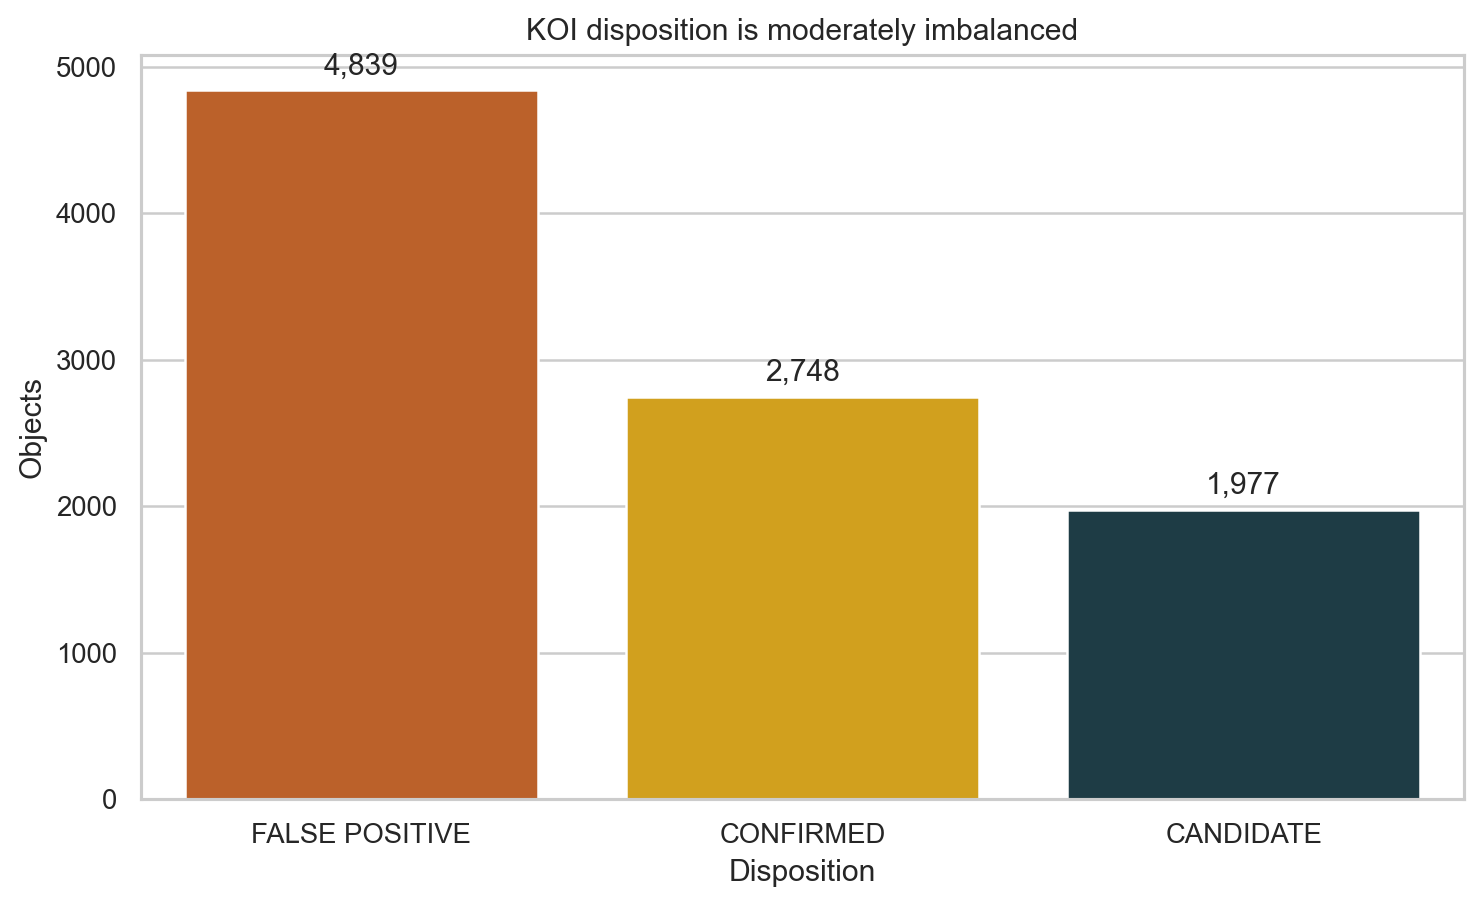
\includegraphics[width=0.72\textwidth]{images/01_target_distribution.png}
\caption{KOI disposition distribution. FALSE POSITIVE is the largest class, so accuracy is not the only evaluation metric.}
\label{fig:koi-target}
\end{figure}

The target counts are 4,839 FALSE POSITIVE objects, 2,748 CONFIRMED objects, and 1,977 CANDIDATE objects. This is a moderate class imbalance. Therefore, the report uses accuracy, balanced accuracy, and macro F1.

Accuracy is the proportion of all correct predictions. It is easy to understand, but it can look high when a model mainly predicts the largest class. Balanced accuracy first calculates recall for each class and then averages those recalls, so a rare class has the same influence as a common class. Macro F1 also gives every class equal weight by averaging its F1 score. F1 combines precision, meaning that a predicted class is correct, and recall, meaning that the model finds the true objects in that class. Using all three numbers gives a more complete view than accuracy alone.

\subsubsection{Data Quality, Missing Values, and Leakage Control}

The data contains missing values in several fields. Some fields are not suitable for prediction because they directly reveal the final decision. For example, the pipeline disposition, confidence score, official Kepler name, and false-positive flags are excluded. Using them would make the test score look better without giving a realistic predictive model.

Missing values mean that a measurement was not available for every catalogue object. A missing value is not automatically an error: a parameter may be absent because it could not be estimated or was not reported in the same way for every object. Figure~\ref{fig:koi-missing} ranks the columns with the highest missing-value share. The plot helps identify which fields would lose too many rows if the analysis simply deleted every incomplete record.

The report does not remove all incomplete rows. Instead, the numerical features used for modelling are filled with a median value and the categorical feature is filled with its most common value. The median is the middle observed value, so it is less affected by very large values than the mean. This choice keeps more training examples while using a simple, explainable rule. The imputation rule is fitted on training data only, as explained later in the preprocessing section.

Leakage is different from missing data. Leakage occurs when an input contains information that would not be available at the time of a real prediction. A field such as an official final name or a false-positive flag can reveal the catalogue outcome directly. Including it would make a model appear strong because it reads the answer indirectly. For this reason, leakage-prone columns are excluded before the split and before training.
\begin{figure}[H]
\centering
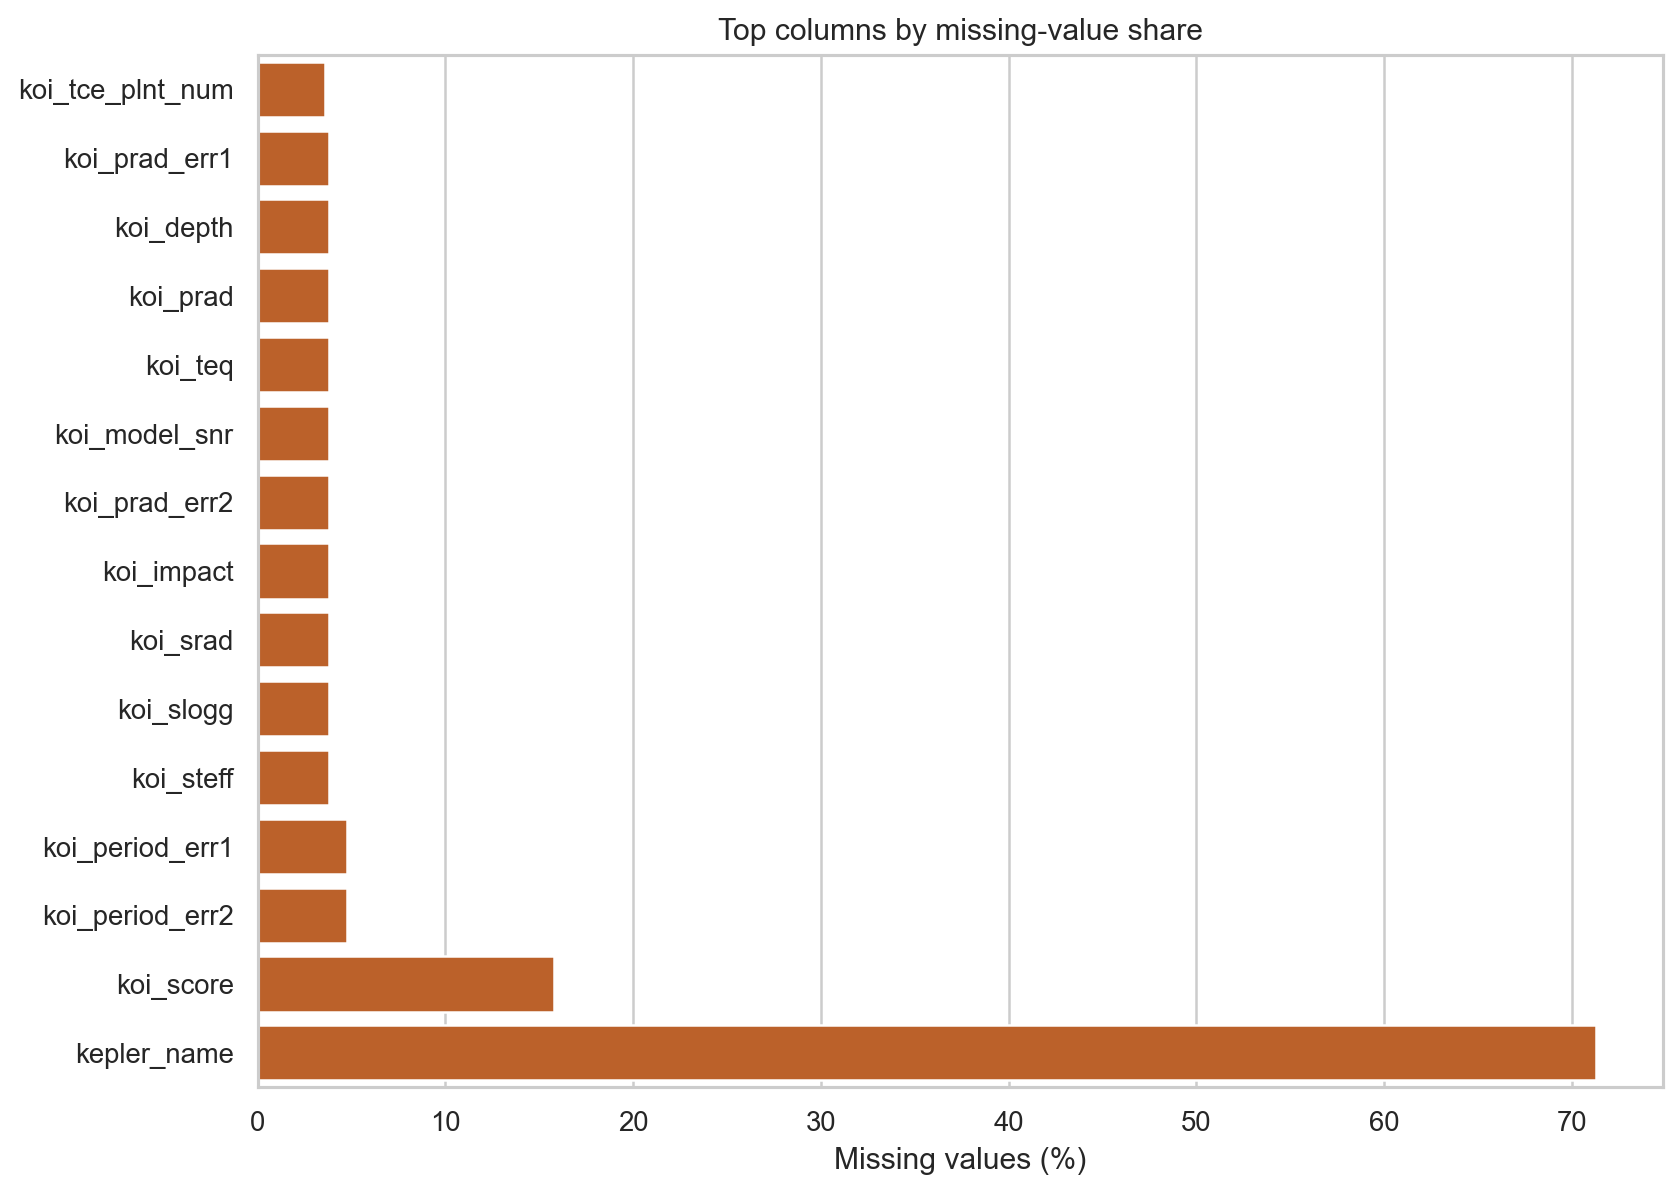
\includegraphics[width=0.75\textwidth]{images/02_missing_values.png}
\caption{Highest missing-value shares among the selected KOI columns.}
\label{fig:koi-missing}
\end{figure}

\subsubsection{Numerical Distributions and Outliers}

Numerical fields such as orbital period and estimated planet radius have long right tails. The plots use a log scale so that both small and large values are visible. Outliers are retained because unusual astronomical objects may still be valid observations.

The histograms in Figure~\ref{fig:koi-distributions} count how many objects fall into ranges of orbital period and planetary radius. A normal horizontal scale would place most short periods or small radii near the left edge and make the large values difficult to see. A logarithmic scale spreads values by orders of magnitude, so both common and rare values can be inspected in one figure. The log scale is used for visualization; the original values are still handled by the preprocessing pipeline.

Outliers are checked with the interquartile range (IQR) rule. For a feature, the first quartile \(Q_1\) is the value below which 25\% of observations lie, and the third quartile \(Q_3\) is the value below which 75\% lie. The IQR is \(Q_3-Q_1\). Values below \(Q_1-1.5\times IQR\) or above \(Q_3+1.5\times IQR\) are counted as possible outliers. Figure~\ref{fig:koi-outliers} reports this share for the selected numerical features. A possible outlier is reviewed, not automatically deleted, because a rare astronomical measurement can still be a valid and informative object.
\begin{figure}[H]
\centering
\begin{minipage}{0.48\textwidth}
\centering
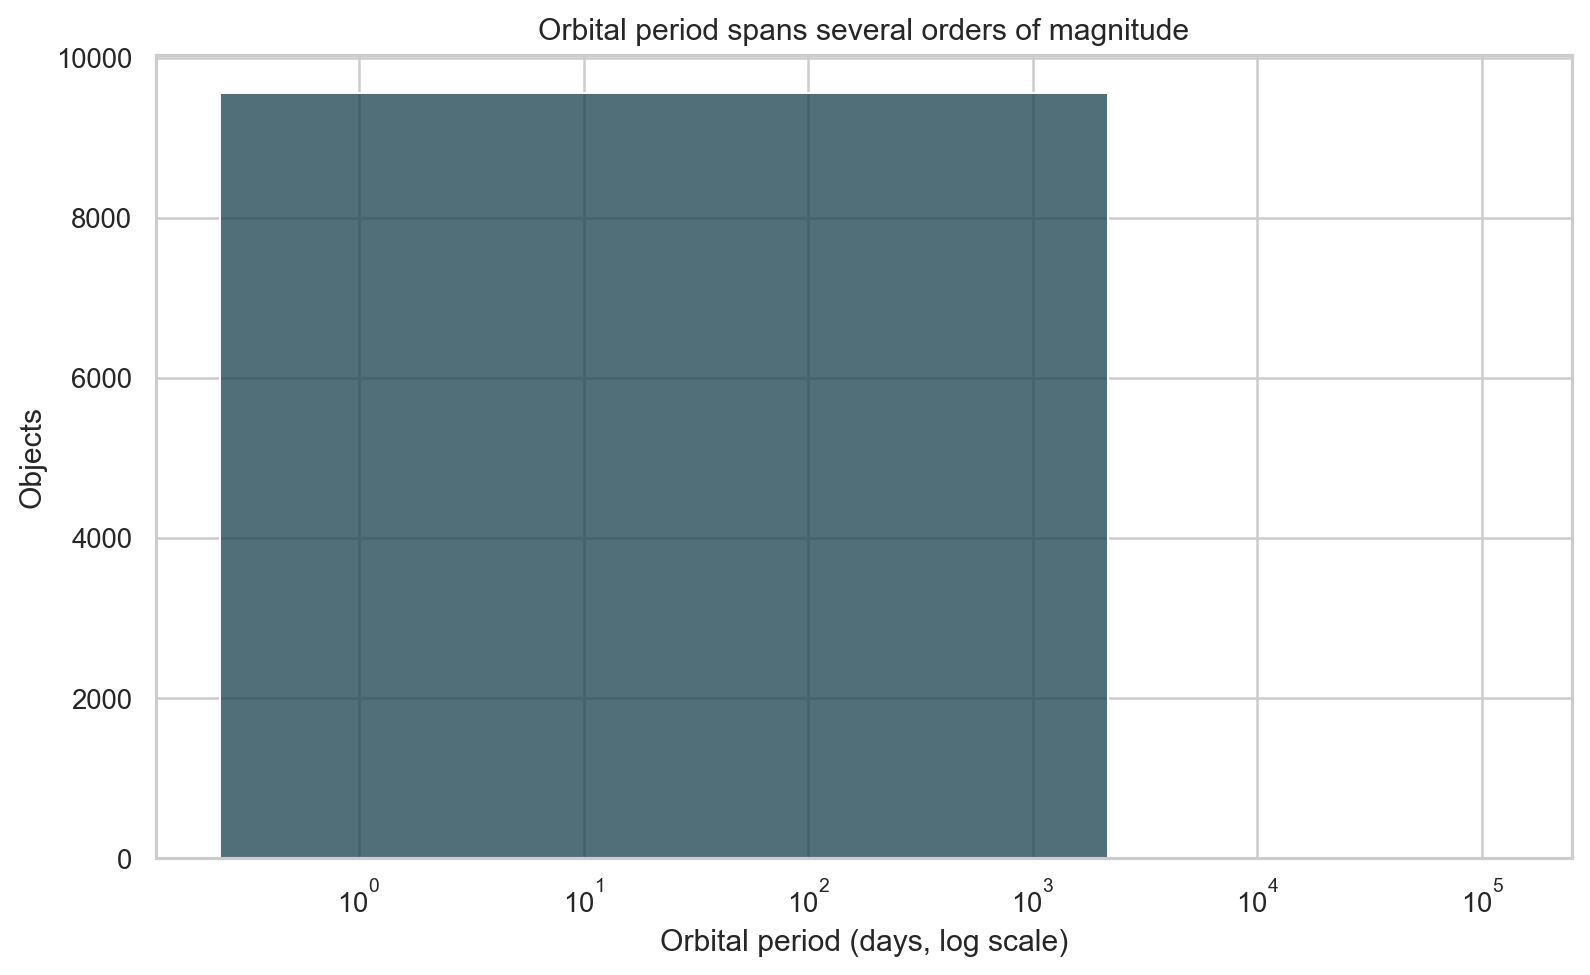
\includegraphics[width=\textwidth]{images/03_orbital_period_distribution.png}\\
\small (a) Orbital period
\end{minipage}\hfill
\begin{minipage}{0.48\textwidth}
\centering
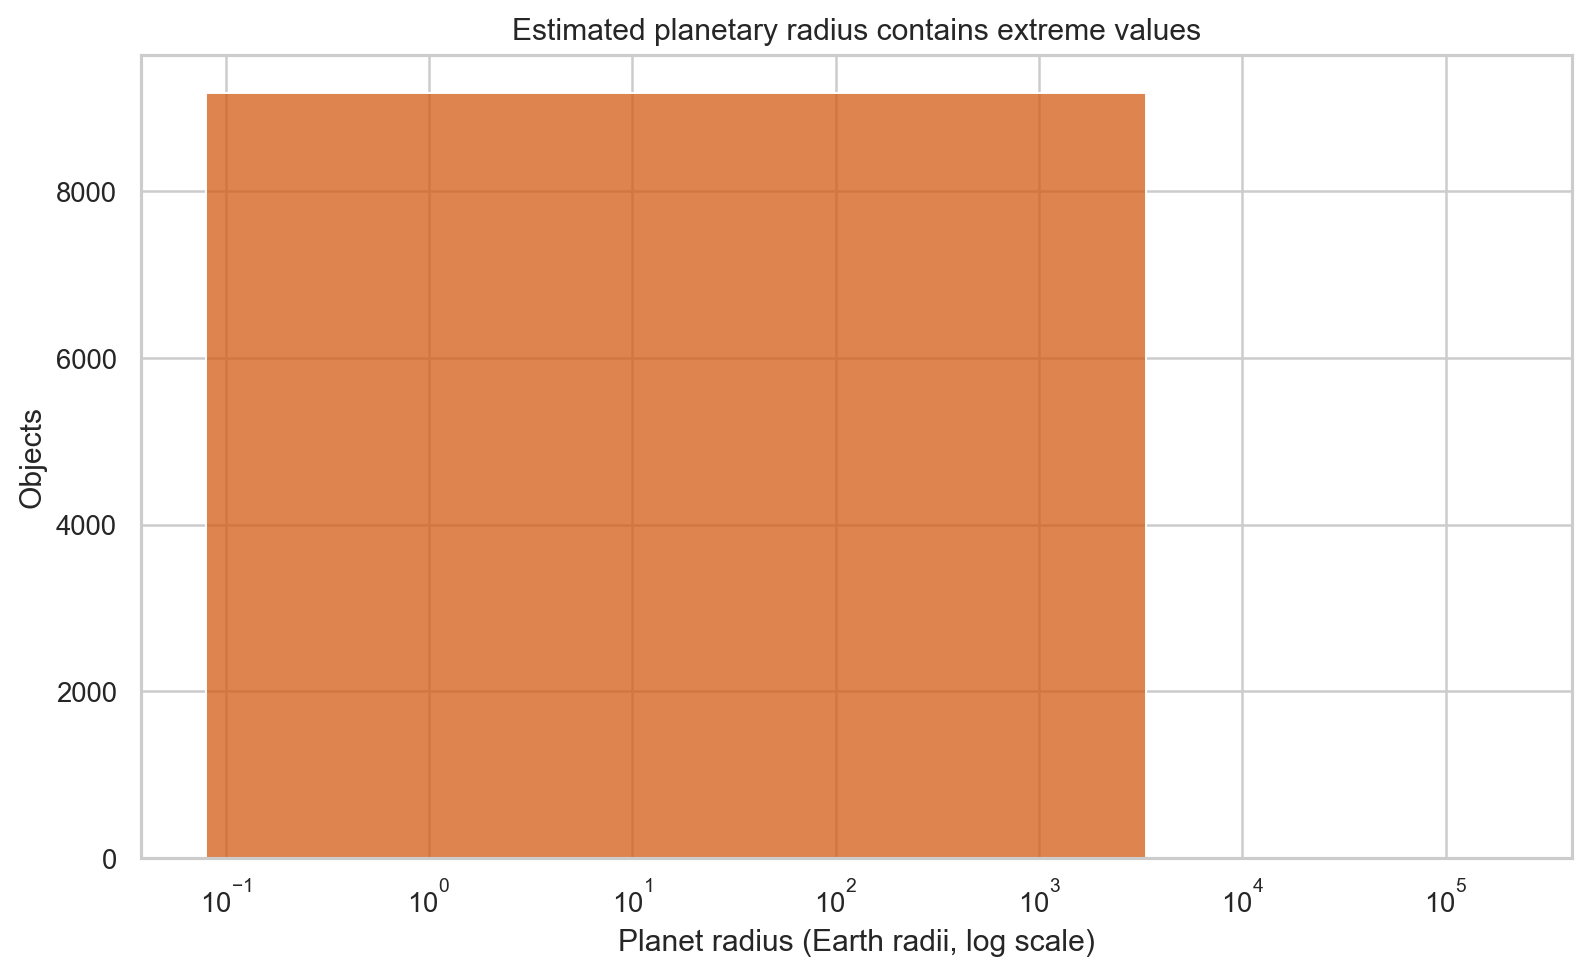
\includegraphics[width=\textwidth]{images/04_planet_radius_distribution.png}\\
\small (b) Planet radius
\end{minipage}
\caption{Two skewed numerical distributions. Log scaling is used for visualization only.}
\label{fig:koi-distributions}
\end{figure}

\begin{figure}[H]
\centering
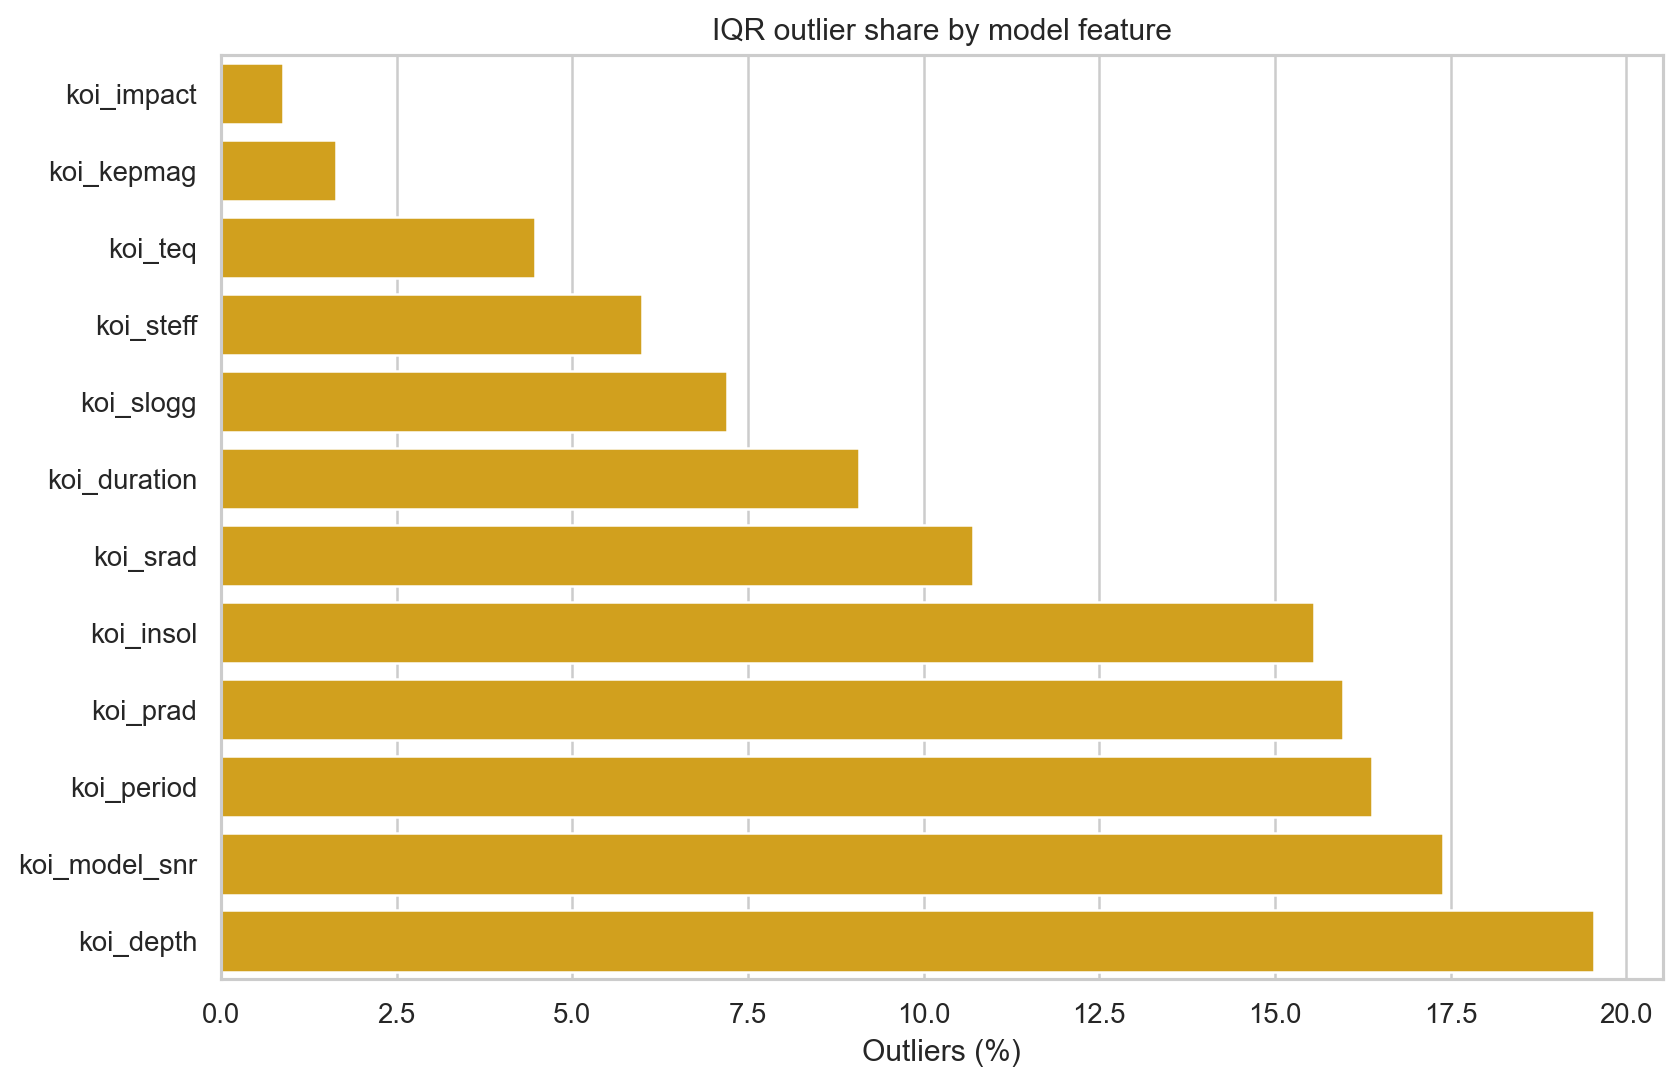
\includegraphics[width=0.72\textwidth]{images/06_outlier_share.png}
\caption{IQR outlier share for numerical model features. Outliers are audited but not deleted.}
\label{fig:koi-outliers}
\end{figure}

\subsubsection{Feature Distributions by KOI Disposition}

The class distributions overlap in every single feature. Figure~\ref{fig:koi-snr} shows this for transit signal-to-noise ratio. A multivariable model is therefore needed.

The boxplots compare the median, central spread, and visible range of a feature for each target class. The most extreme one percent of values is hidden only in these comparison plots so that the central patterns can be read clearly; those rows are not removed from the dataset. The overlap shows that a simple rule based on radius alone would make many mistakes. The model needs several measurements together, because a useful pattern may be created by the combination of radius, period, signal strength, and other features.
\begin{figure}[H]
\centering
\begin{minipage}{0.48\textwidth}
\centering
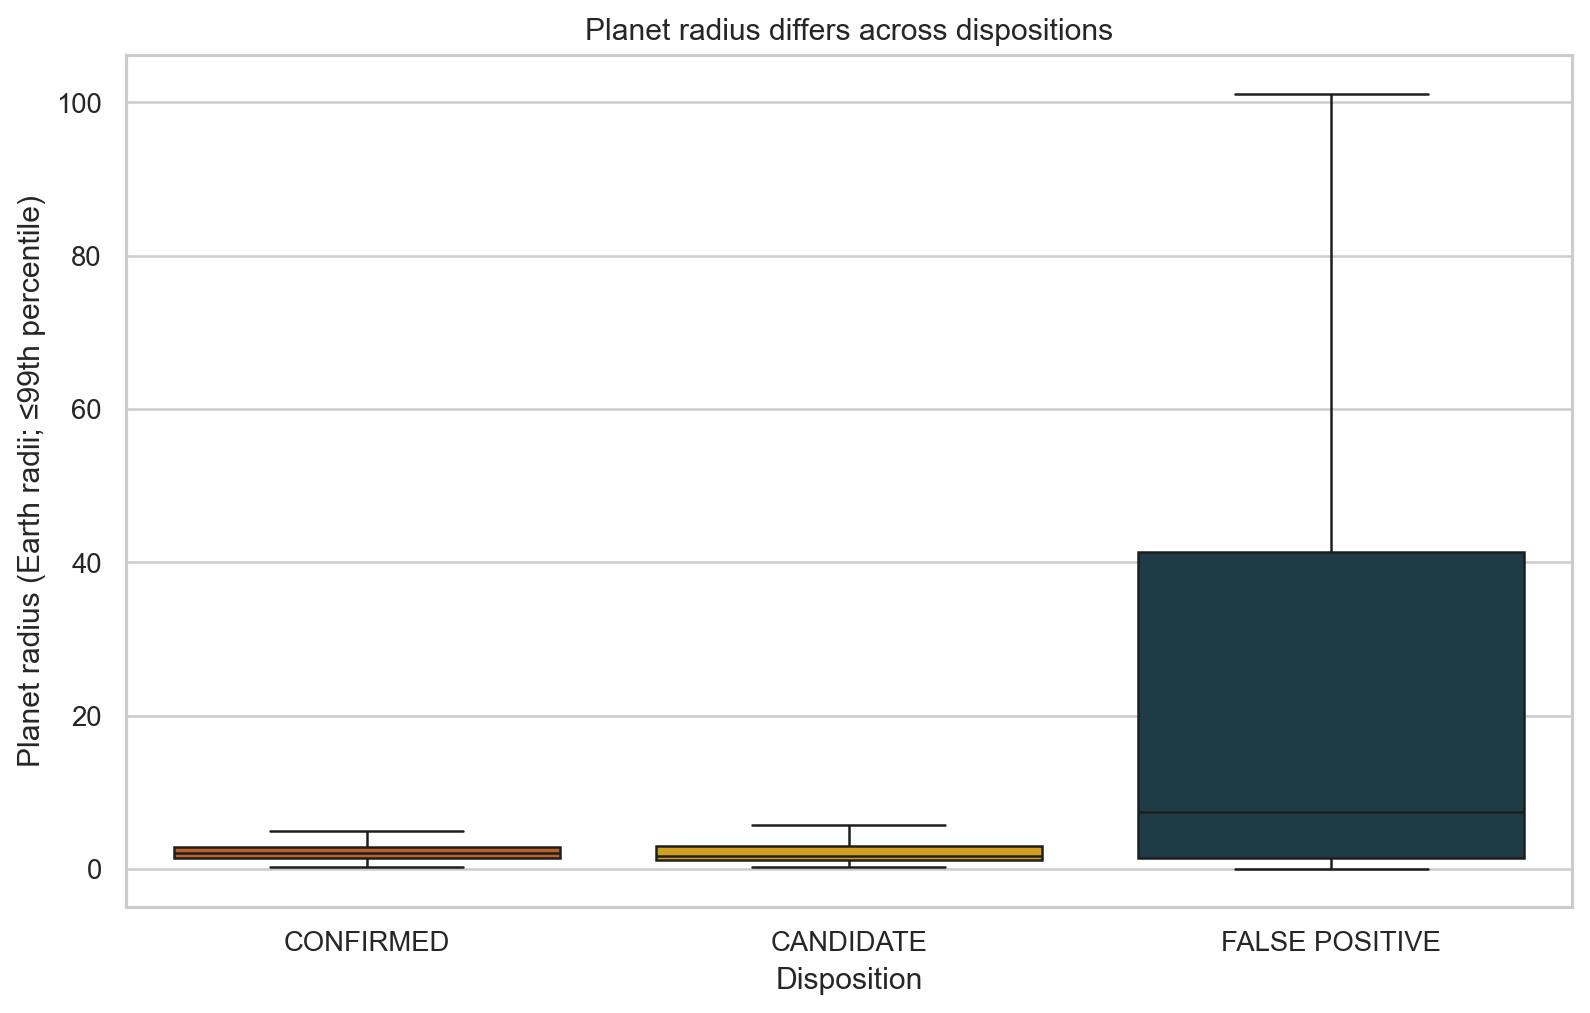
\includegraphics[width=\textwidth]{images/07_target_vs_planet_radius.png}\\
\small (a) Planet radius by disposition
\end{minipage}\hfill
\begin{minipage}{0.48\textwidth}
\centering
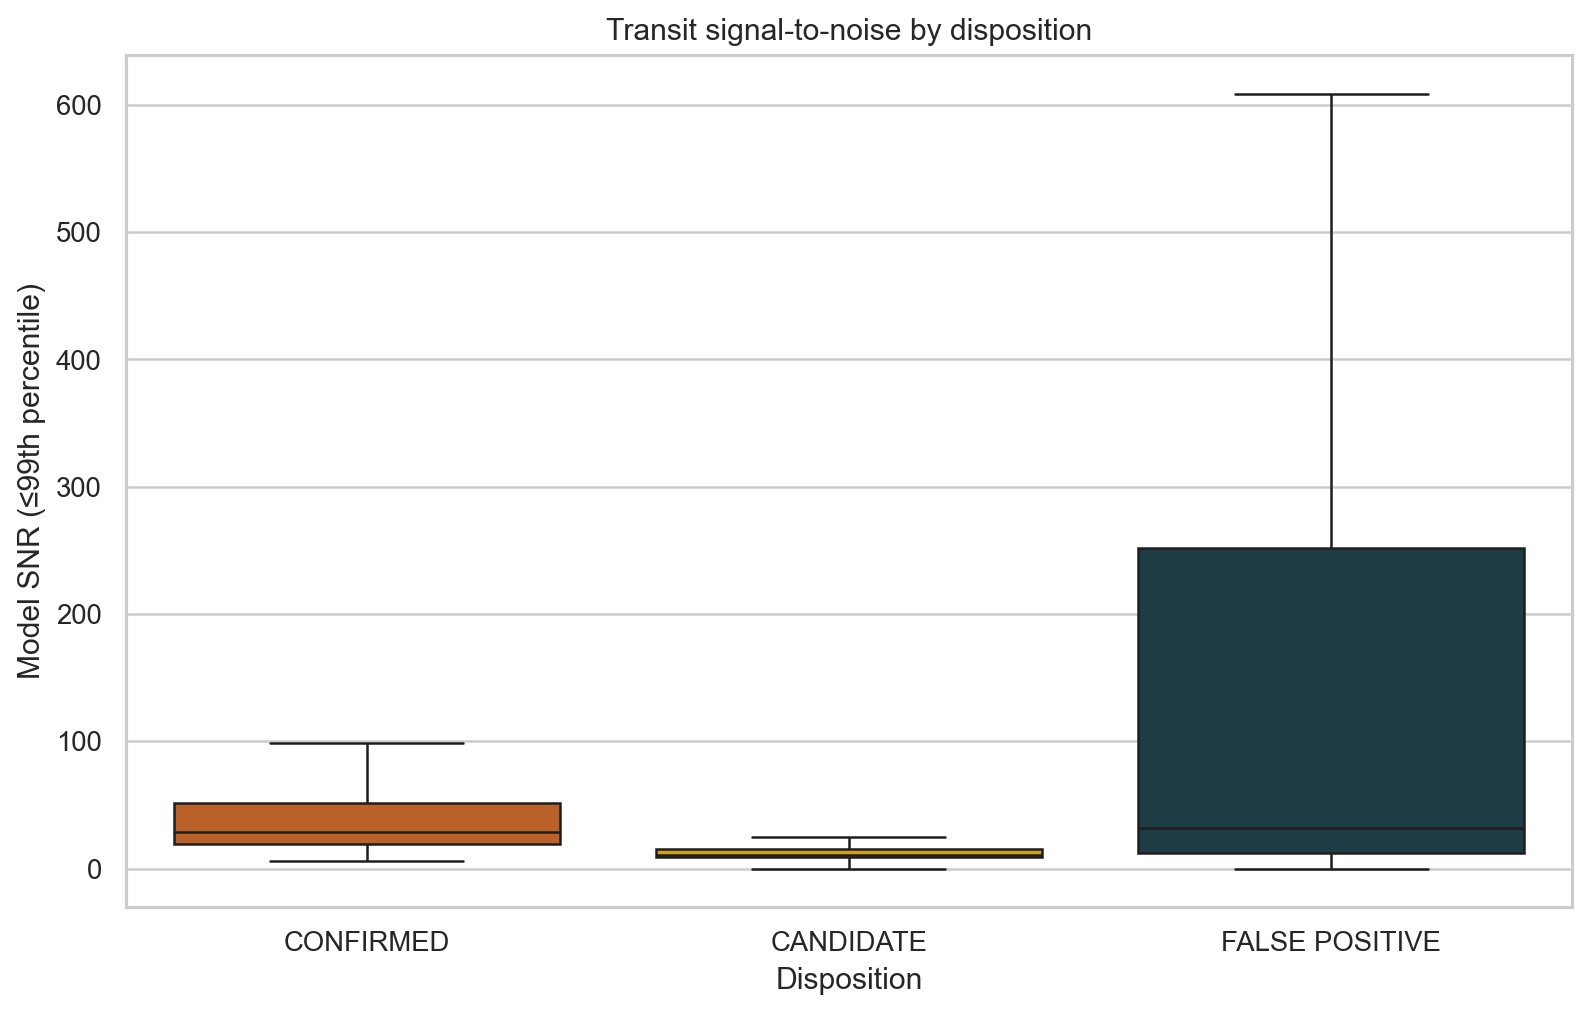
\includegraphics[width=\textwidth]{images/08_target_vs_snr.png}\\
\small (b) Signal-to-noise ratio by disposition
\end{minipage}
\caption{Class-conditional distributions for two useful features. The overlap prevents a rule based on one column.}
\label{fig:koi-snr}
\end{figure}

\subsection{Preprocessing and Evaluation Design}

\subsubsection{Feature Preparation}

The final model uses 12 numerical features and one categorical feature, \texttt{koi\_tce\_delivname}. Numerical missing values are imputed with the median. The categorical field is filled with the most common value and one-hot encoded. Logistic Regression uses standard scaling. Random Forest uses robust scaling in the same preprocessing pipeline.

The feature list is selected before modelling. The twelve numerical columns describe measurable properties of the signal and its host star. The categorical column identifies the TCE delivery catalogue. One-hot encoding turns each possible catalogue value into its own 0-or-1 indicator column. This lets a model use a category without treating its text name as a number with an artificial order.

The preprocessing pipeline has a fixed order. First, it receives only the selected columns. Second, it fills missing numerical values with the training median and missing category values with the training mode. Third, it scales numerical values and one-hot encodes the category. Finally, it sends the transformed feature matrix to the classifier. Keeping these steps in a Scikit-learn pipeline prevents an accidental difference between training data and evaluation data.

Standard scaling subtracts a feature mean and divides by its standard deviation, so features measured in days, radii, or kelvin have comparable sizes for Logistic Regression. Robust scaling uses the median and IQR instead, so a few extreme observations have less influence on the transformation. Tree models do not require scaling to make their splits, but the robust scaler is retained in the Random Forest pipeline to keep the numerical preparation stable and explicit. In both cases, the scaler learns its values from the training split only.

\subsubsection{Group-Aware Train, Validation, and Test Split}

The split is based on \texttt{kepid}, the host-star identifier. A GroupShuffleSplit separates data into 70\% train, 15\% validation, and 15\% test. This prevents objects from the same star from appearing in more than one split.

The split is done in two steps. First, 30\% of the host-star groups are held aside. Second, that held-aside part is divided equally into validation and test groups. The result is approximately 70\% training, 15\% validation, and 15\% testing data. The word approximately is important because a group may contain more than one KOI object, so the exact row count is determined by groups rather than by individual rows.

This group-aware split is stricter than a random row split. If several signals from the same star appeared in both training and testing data, the model could benefit from star-specific information that it has already seen. Grouping by \texttt{kepid} makes the test closer to the real question: can the model classify signals from host stars that were not used for training?

\begin{figure}[H]
\centering
\begin{minipage}{0.48\textwidth}
\centering
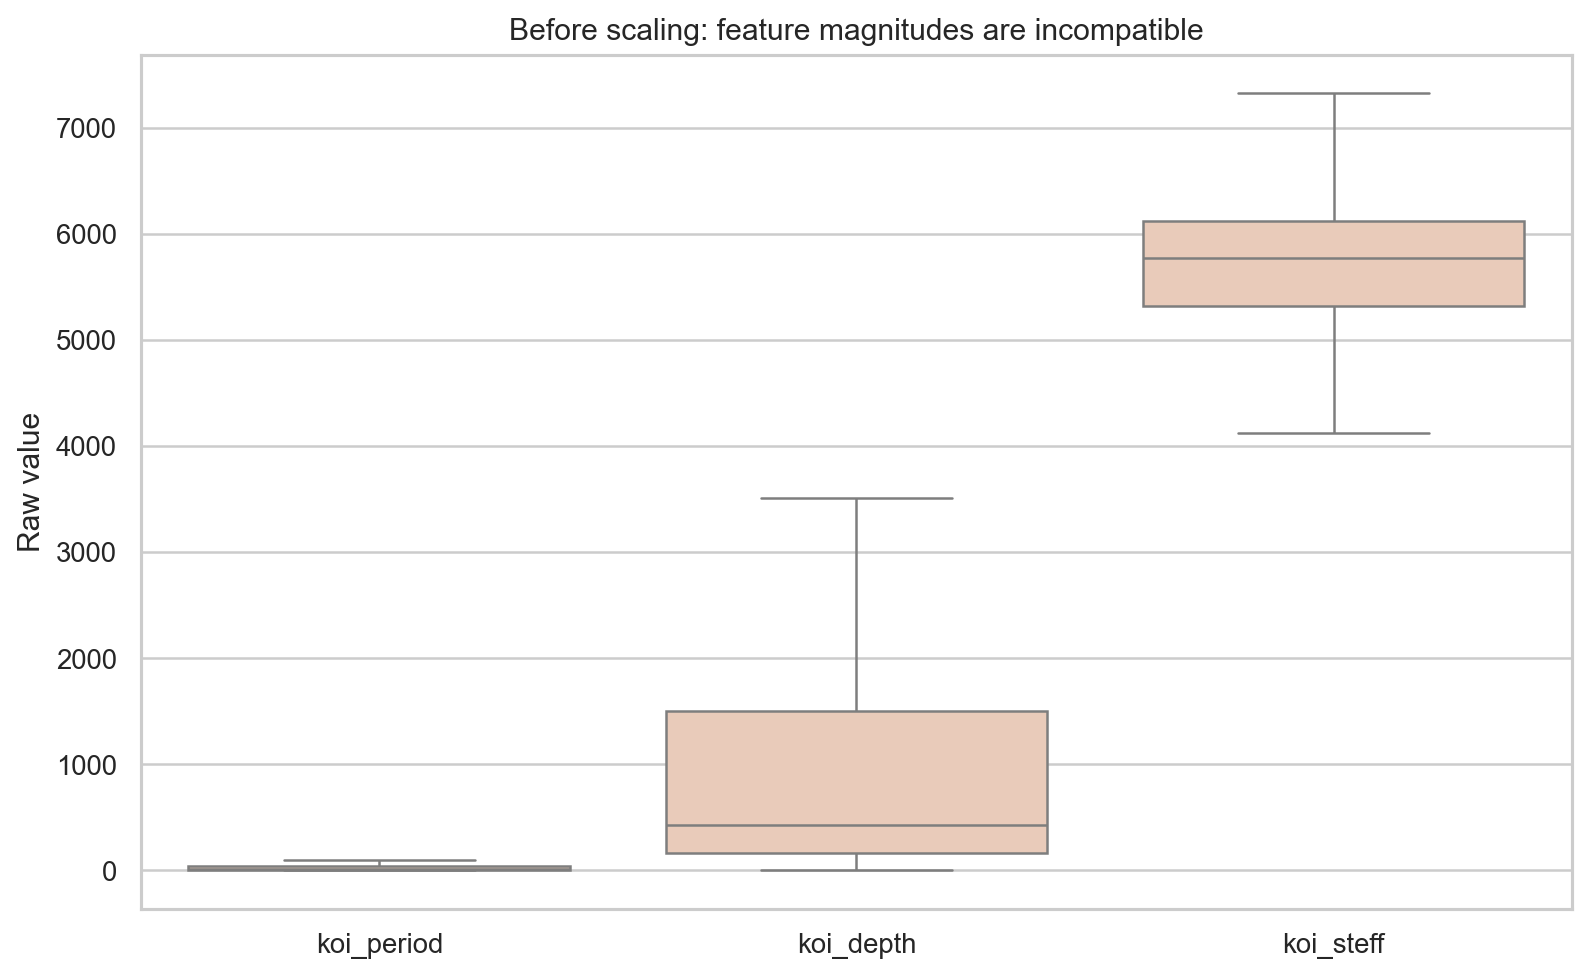
\includegraphics[width=\textwidth]{images/10_before_scaling.png}\\
\small (a) Before scaling
\end{minipage}\hfill
\begin{minipage}{0.48\textwidth}
\centering
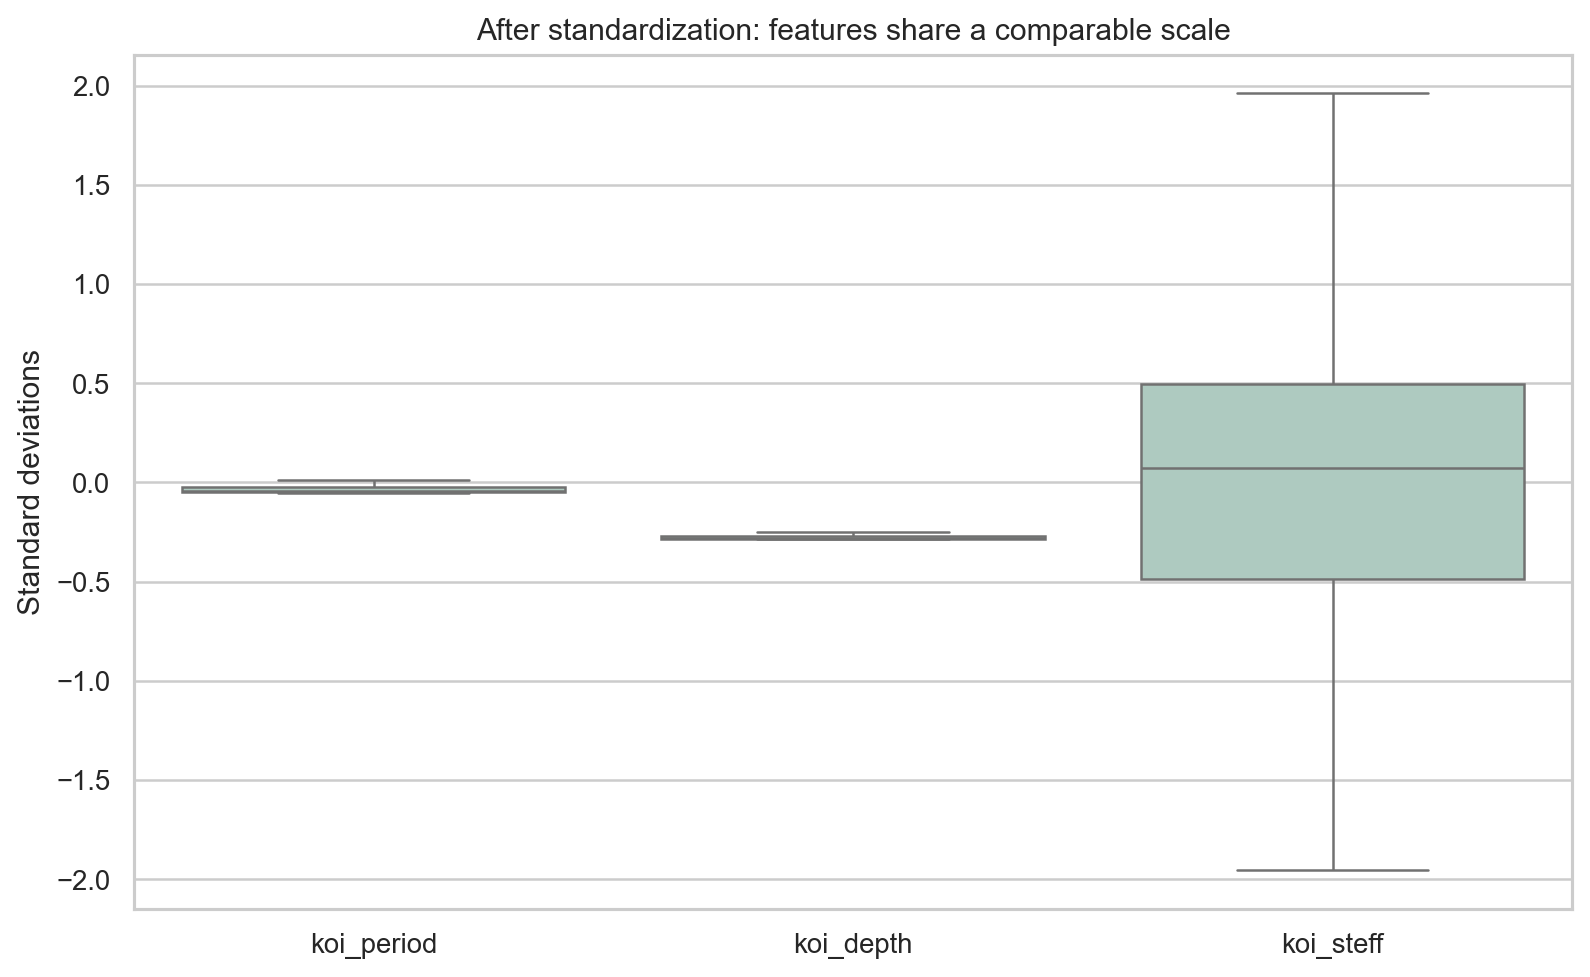
\includegraphics[width=\textwidth]{images/11_after_scaling.png}\\
\small (b) After standardization
\end{minipage}
\caption{Scaling illustration for three numerical variables. The actual transforms are fitted using training data only.}
\label{fig:koi-scaling}
\end{figure}

\subsection{Model Comparison and Final Evaluation}

\subsubsection{Baseline and Balanced Random Forest}

Two models are compared on the validation split. Logistic Regression is the simple linear baseline. The final model is a Random Forest with 350 trees, balanced class weights, and a minimum leaf size of 2. Macro F1 is used to select the final model because it gives all three classes equal weight.

Logistic Regression is used first because it is a simple and interpretable baseline. For each class, it combines the prepared feature values with learned weights and produces a class score. A positive or negative weight changes the score, but the model can only form a linear boundary in the transformed feature space. If the relationship between measurements and the class is more complex, this baseline may be too simple.

Random Forest is an ensemble of decision trees. Each tree repeatedly asks a simple question, for example whether a measurement is below a learned threshold. The trees are trained with different samples and different subsets of features, then vote for the final class. Combining many trees can capture non-linear relationships and interactions between features. The minimum leaf size of 2 stops a tree from creating a final decision from only one row, and 350 trees make the voting result more stable.

The \texttt{class\_weight} setting uses the balanced subsample option to give more importance to under-represented classes inside each tree sample. It does not create new KOI objects. Instead, an error on a less common class has a larger training cost, which encourages the forest to pay attention to CONFIRMED and CANDIDATE objects as well as the large FALSE POSITIVE class.
\subsubsection{Validation Model Comparison}

\begin{table}[H]
\centering
\caption{Validation results for the tabular task.}
\label{tab:koi-validation}
\begin{tabular}{lrrr}
\toprule
\textbf{Model} & \textbf{Accuracy} & \textbf{Balanced accuracy} & \textbf{Macro F1} \\
\midrule
Logistic Regression & 0.660 & 0.582 & 0.558 \\
Balanced Random Forest & \textbf{0.788} & \textbf{0.759} & \textbf{0.758} \\
\bottomrule
\end{tabular}
\end{table}

\begin{figure}[H]
\centering
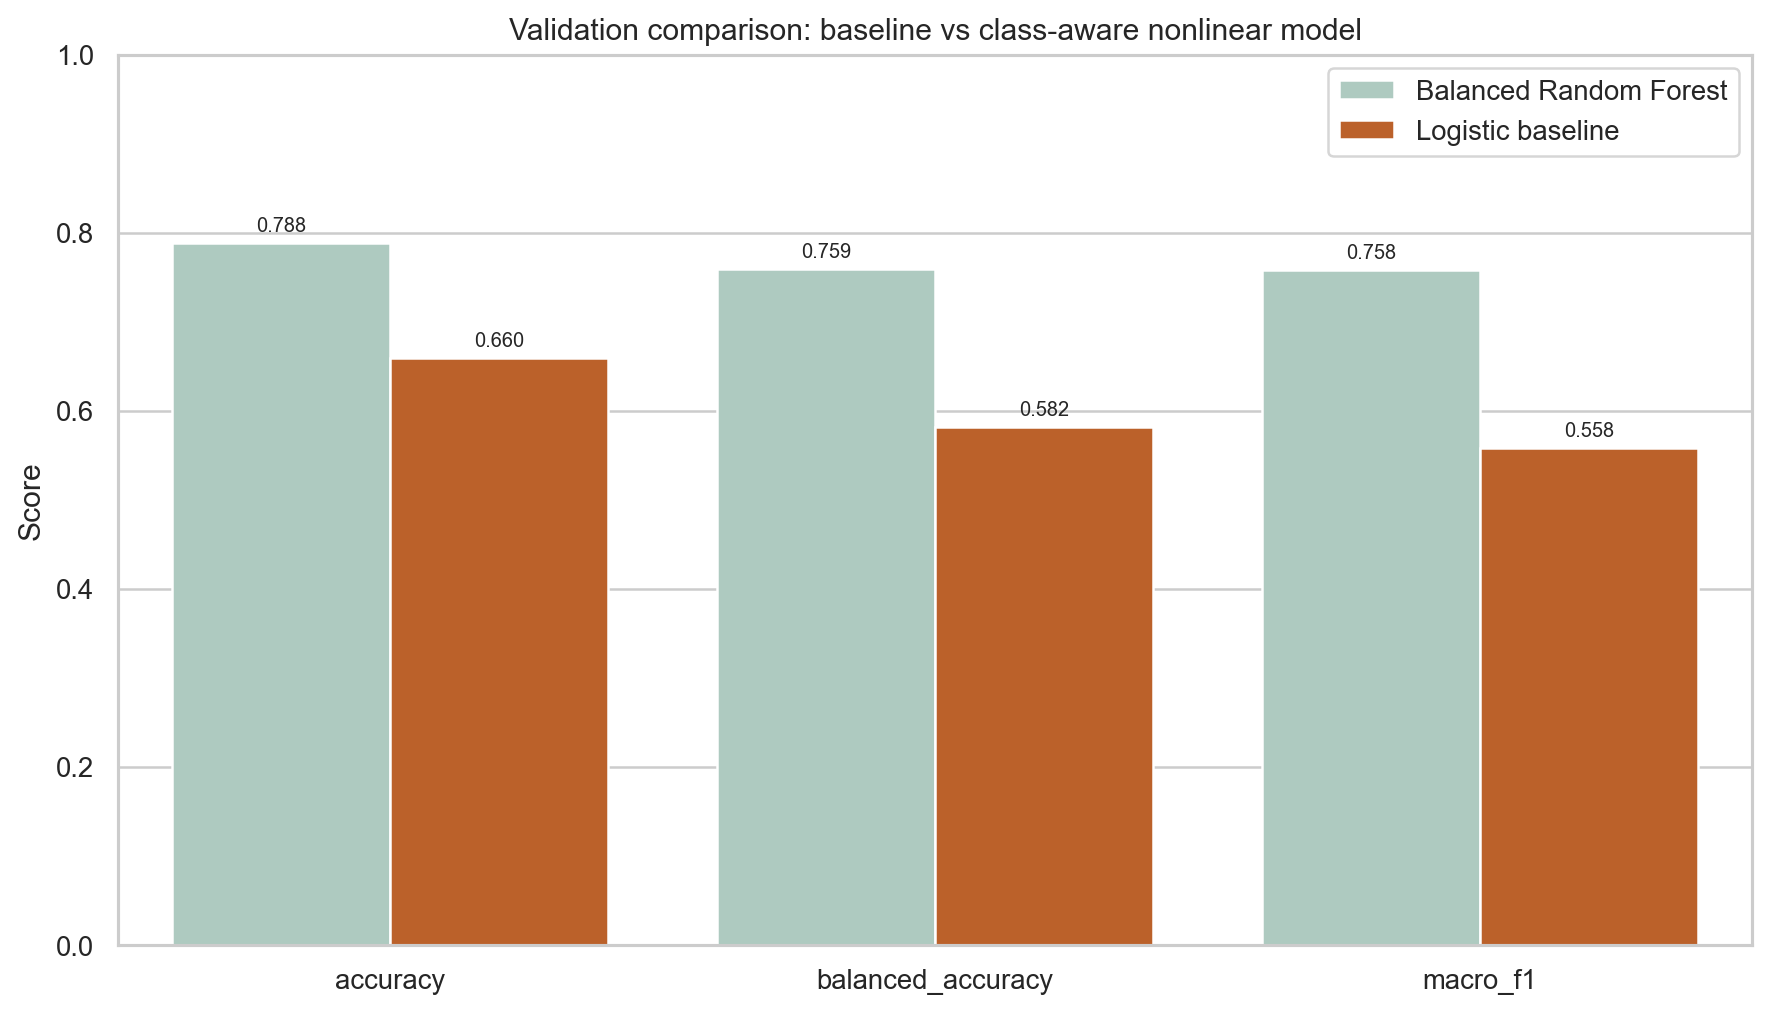
\includegraphics[width=0.78\textwidth]{images/12_model_comparison.png}
\caption{Validation comparison. The class-aware Random Forest improves all three metrics.}
\label{fig:koi-model-comparison}
\end{figure}

\noindent The validation table should be read as a model-selection result, not as the final claim. The Random Forest is higher on all three validation measures. In particular, its macro F1 is much higher than the Logistic Regression baseline, so the improvement is not only caused by making more correct predictions for the largest class. This is why the forest, rather than the baseline, is carried to the final test.

\subsubsection{Final Test Results and Feature Importance}

The selected model is evaluated once on the test split. It reaches 0.758 accuracy, 0.730 balanced accuracy, and 0.727 macro F1. The candidate class is the most difficult class, which is expected because it lies between confirmed planets and false positives.

The test split is not used to choose hyperparameters or to change the feature list. It is used once after validation has selected the Random Forest. This separation is important: repeatedly looking at test results and changing the model would make the final score too optimistic.

The normalized confusion matrix in Figure~\ref{fig:koi-final} is read row by row. A row represents the true class and a column represents the predicted class. Values on the diagonal are correct predictions for that class. Values outside the diagonal show which classes are confused. The CANDIDATE row is harder because candidates can share measurement patterns with both confirmed objects and false positives. The matrix therefore explains an important limitation that a single accuracy number cannot show.

Permutation importance provides a second explanation of the selected model. For one feature at a time, the values in the test set are shuffled eight times while all other columns remain unchanged. If macro F1 decreases after that shuffle, the model was using that feature. A large decrease means the feature was useful to the current model on unseen host stars. This is a model-based importance score, not scientific proof that the feature causes the catalogue decision.

\begin{figure}[H]
\centering
\begin{minipage}{0.49\textwidth}
\centering
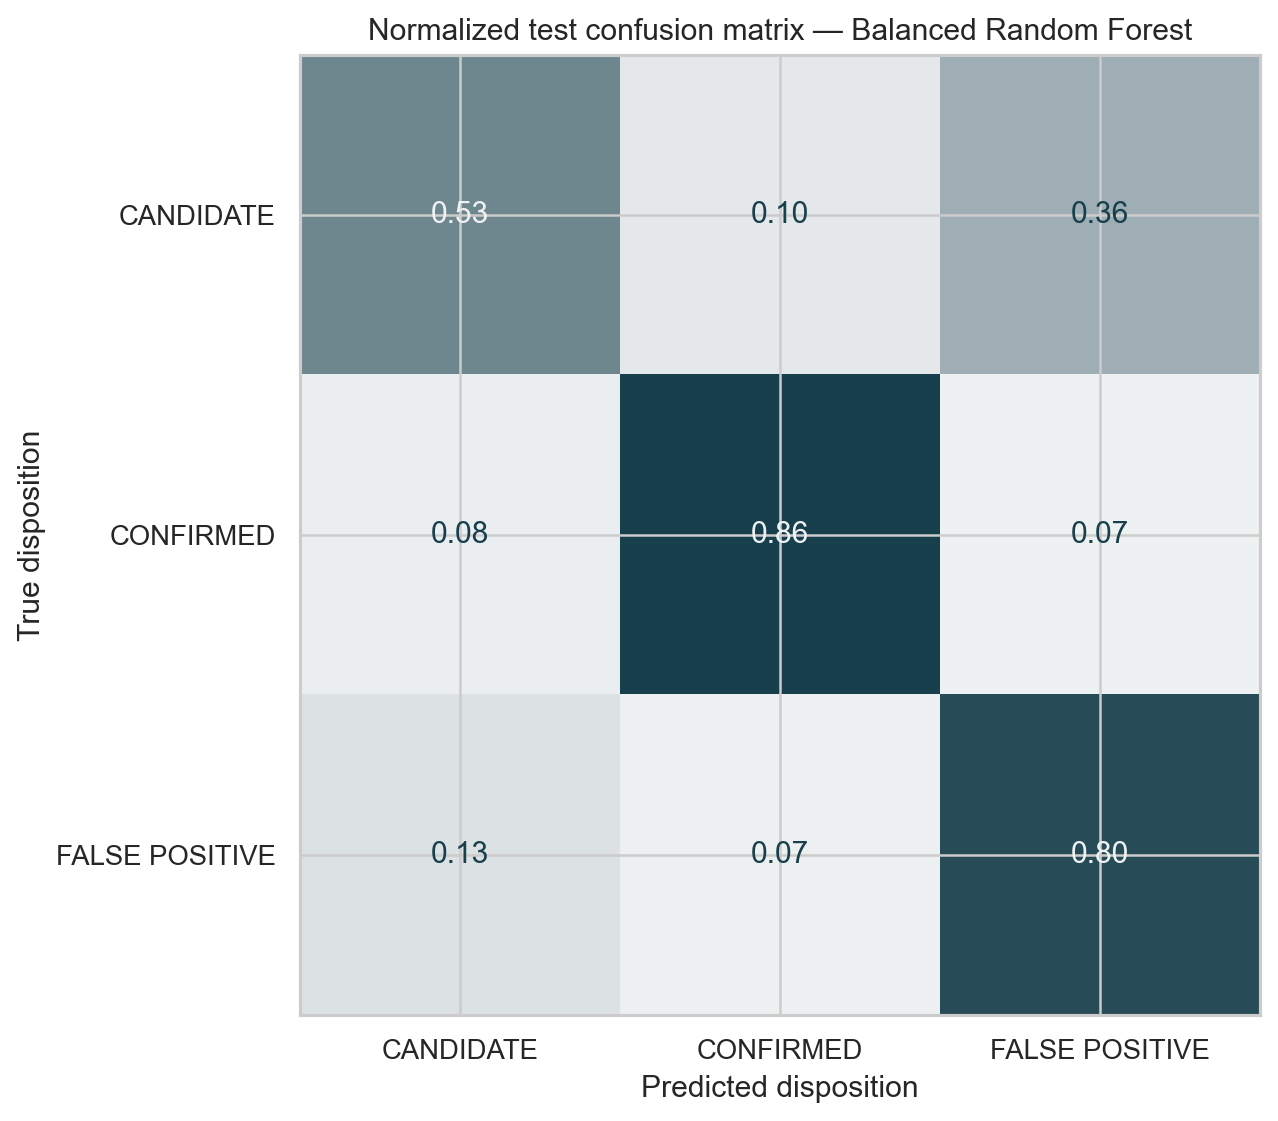
\includegraphics[width=\textwidth]{images/13_confusion_matrix.png}\\
\small (a) Normalized test confusion matrix
\end{minipage}\hfill
\begin{minipage}{0.49\textwidth}
\centering
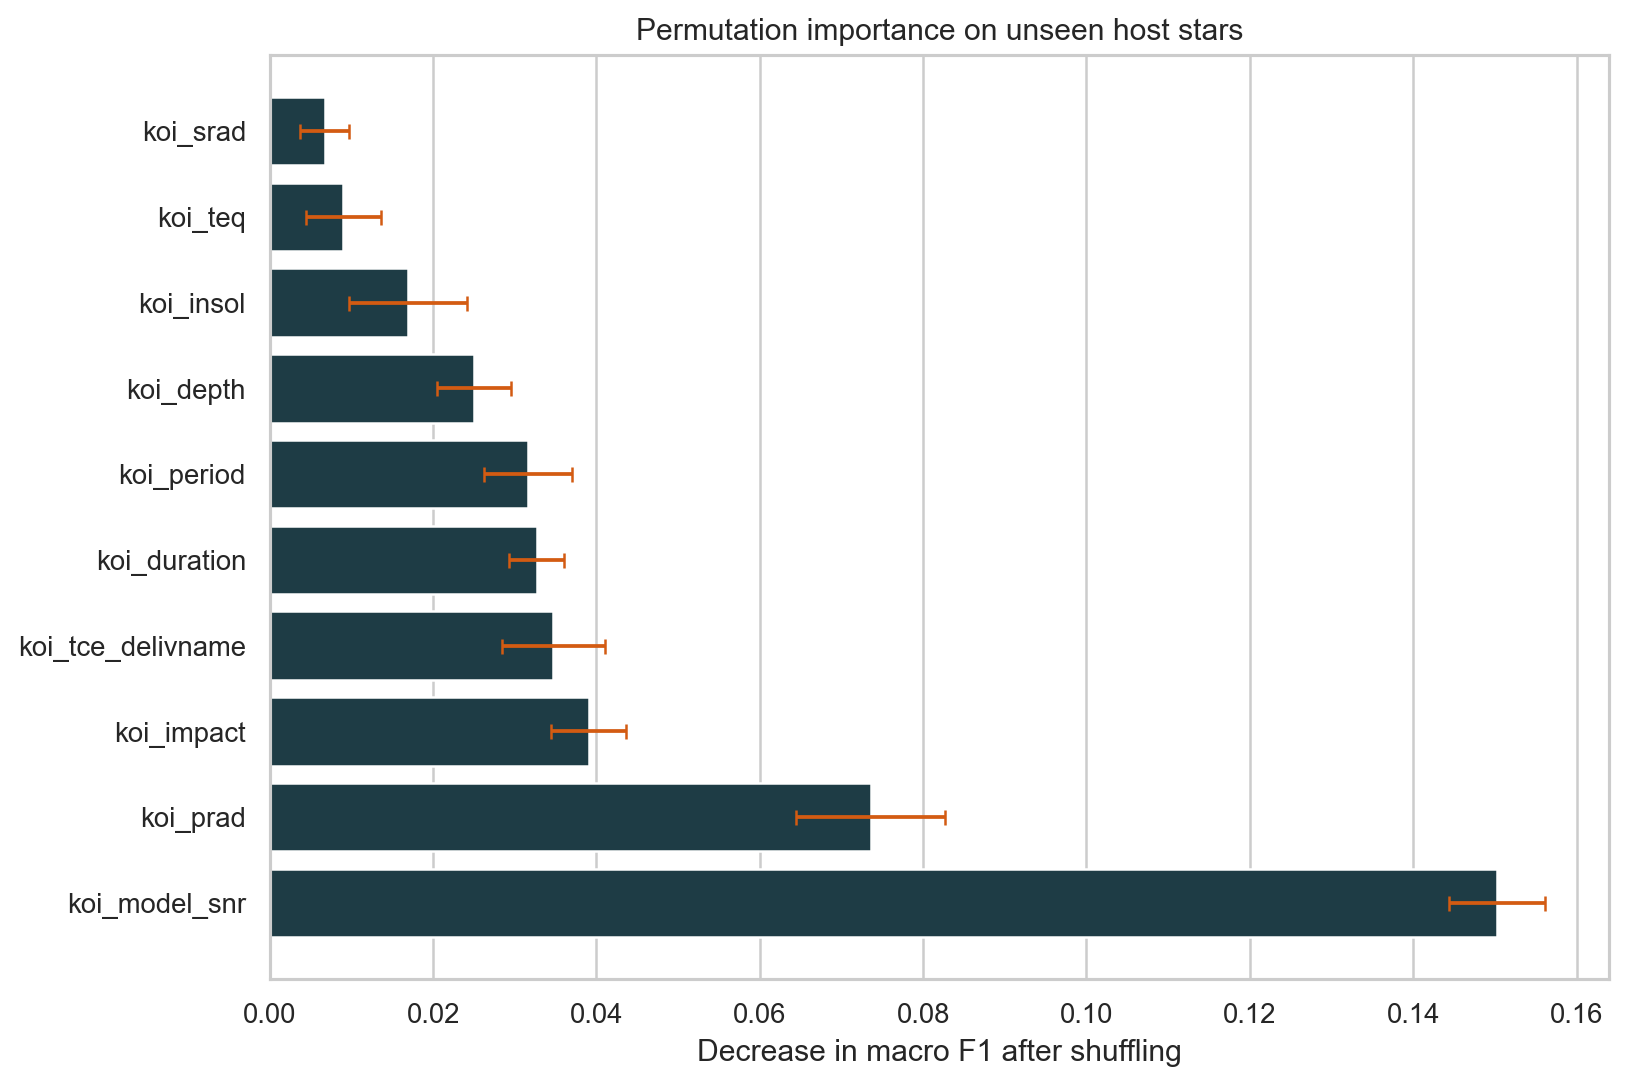
\includegraphics[width=\textwidth]{images/14_feature_importance.png}\\
\small (b) Permutation importance
\end{minipage}
\caption{Final test evaluation and feature importance for the Random Forest.}
\label{fig:koi-final}
\end{figure}

The three strongest features are \texttt{koi\_model\_snr}, \texttt{koi\_prad}, and \texttt{koi\_impact}. This does not prove a causal relationship. It only indicates that shuffling each feature reduces the model's macro F1 on unseen data.

The result is consistent with the earlier EDA: signal quality, estimated planetary radius, and transit geometry help separate the three catalogue labels. However, importance values should be interpreted carefully. Correlated measurements can share information, so one feature may look less important when another related feature is also present. The ranking is useful for explaining the trained classifier, not for replacing domain-specific astronomy analysis.
\subsubsection{Key Findings and Limitations}

\begin{importantbox}
\textbf{Tabular conclusion.} The dataset contains missing values, class imbalance, skewness, and outliers. The Random Forest is better than the linear baseline on the validation split. However, it is a catalogue classifier, not a system that can confirm a planet. Scientific confirmation still needs physical validation and follow-up observations.
\end{importantbox}

\clearpage
\section{Text Data: ViCTSD Vietnamese Comments}
\label{sec:text}

\subsection{Exploratory Data Analysis}

\subsubsection{Dataset Size, Official Split, and Labels}

The text task uses the official Vietnamese Constructive and Toxic Speech Detection dataset (ViCTSD) \cite{victsd}. The source contains 10,000 Vietnamese social-media comments from ten news topics. Each comment has two binary labels: Toxicity and Constructiveness.

The two labels answer two different questions. The toxicity label asks whether a comment contains harmful or offensive language. The constructiveness label asks whether a comment contributes to a useful and respectful discussion. They are not treated as opposite labels in this report. A comment can be analysed by a toxicity model and by a constructiveness model separately, because the two targets describe different aspects of the same text.

\begin{table}[H]
\centering
\caption{ViCTSD dataset summary.}
\label{tab:victsd-summary}
\begin{tabular}{lr}
\toprule
\textbf{Item} & \textbf{Value} \\
\midrule
All comments & 10,000 \\
Topics & 10 \\
Official train split & 7,000 \\
Official validation split & 2,000 \\
Official test split & 1,000 \\
Toxic comments & 1,101 (11.01\%) \\
Exact duplicate comments & 65 \\
\bottomrule
\end{tabular}
\end{table}

\begin{figure}[H]
\centering
\begin{minipage}{0.47\textwidth}
\centering
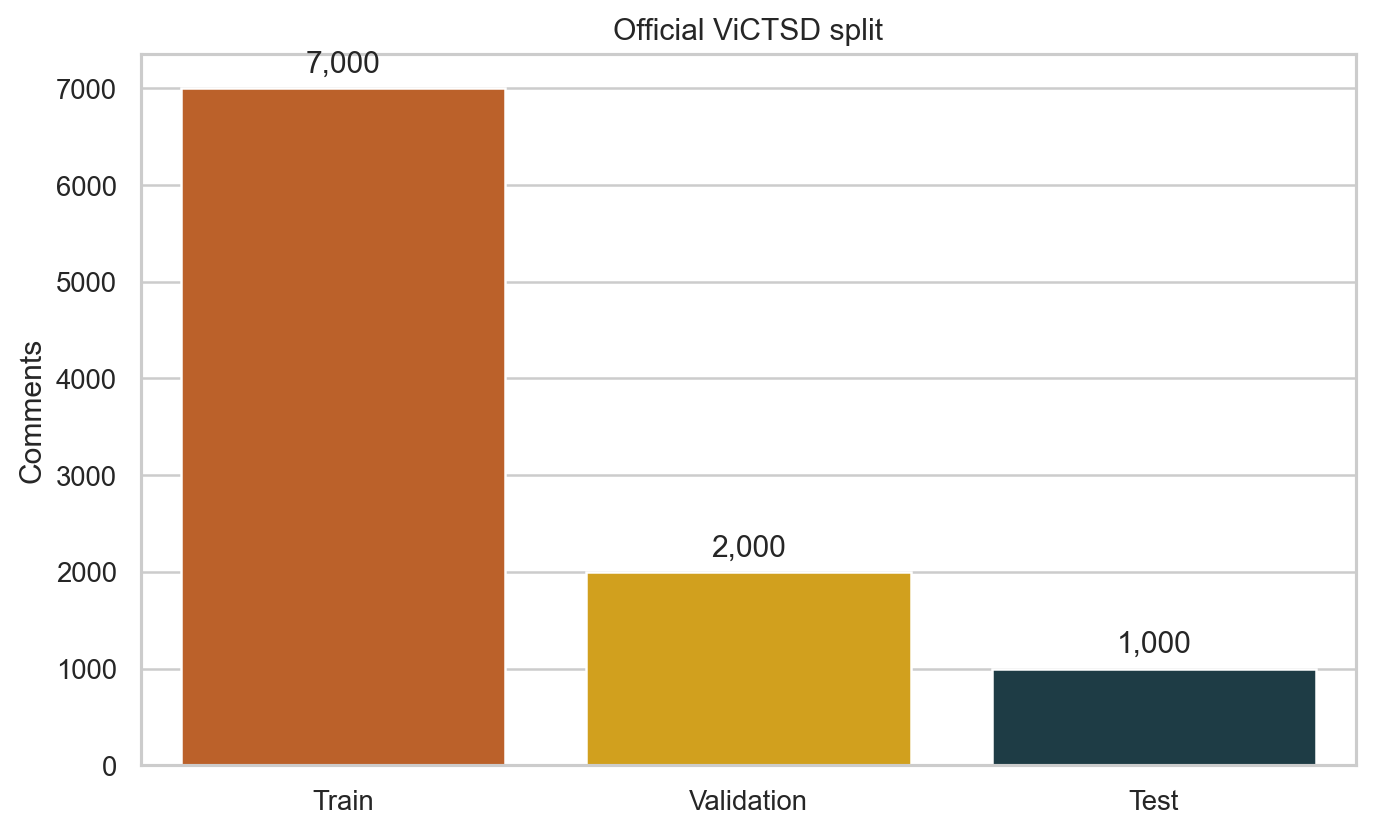
\includegraphics[width=\textwidth]{images/text_01_split_sizes.png}\\
\small (a) Official split
\end{minipage}\hfill
\begin{minipage}{0.47\textwidth}
\centering
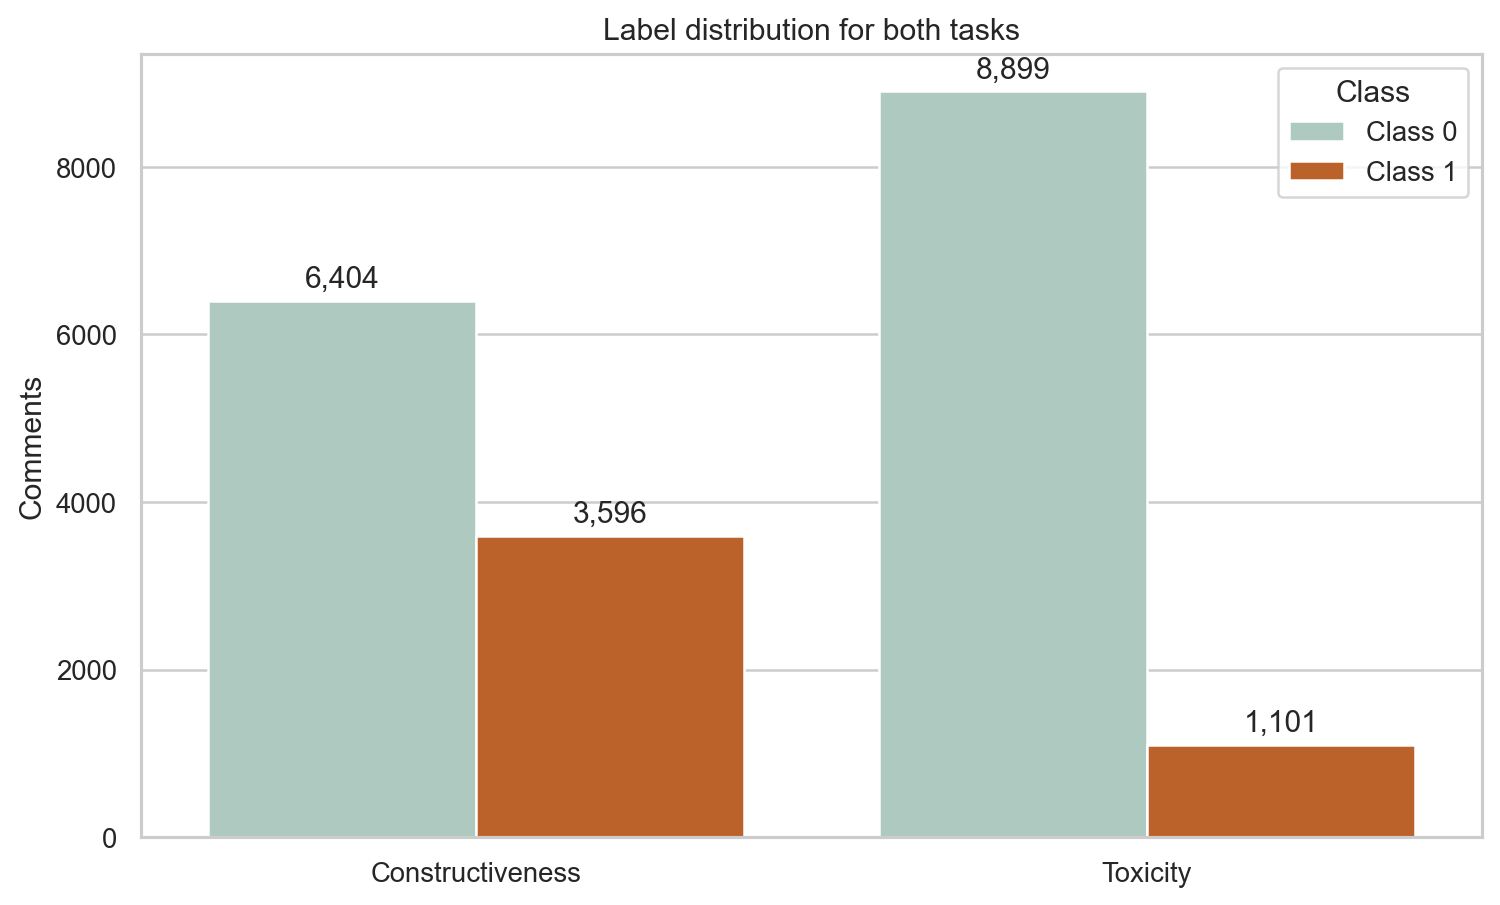
\includegraphics[width=\textwidth]{images/text_02_label_distribution.png}\\
\small (b) Label distribution
\end{minipage}
\caption{Official ViCTSD split and label distributions. Toxicity is the more imbalanced task.}
\label{fig:text-overview}
\end{figure}

The official split is preserved as the starting point. The training split is used to learn the text representation and model coefficients. The validation split is used to compare simple model choices. The test split is kept for one final evaluation after the choice is made. This order prevents the final score from influencing everyday modelling decisions.

\subsubsection{Topic Balance and Comment Length}

The topics are balanced: each topic contributes 1,000 comments. This is useful for exploration because one topic cannot dominate the basic count plots. Topic and article title are not used as model inputs. The first model only uses the comment text. This keeps the prediction question clear: the model should learn from the words in a comment, not from a topic name that may happen to have a different label pattern.

\begin{figure}[H]
\centering
\begin{minipage}{0.47\textwidth}
\centering
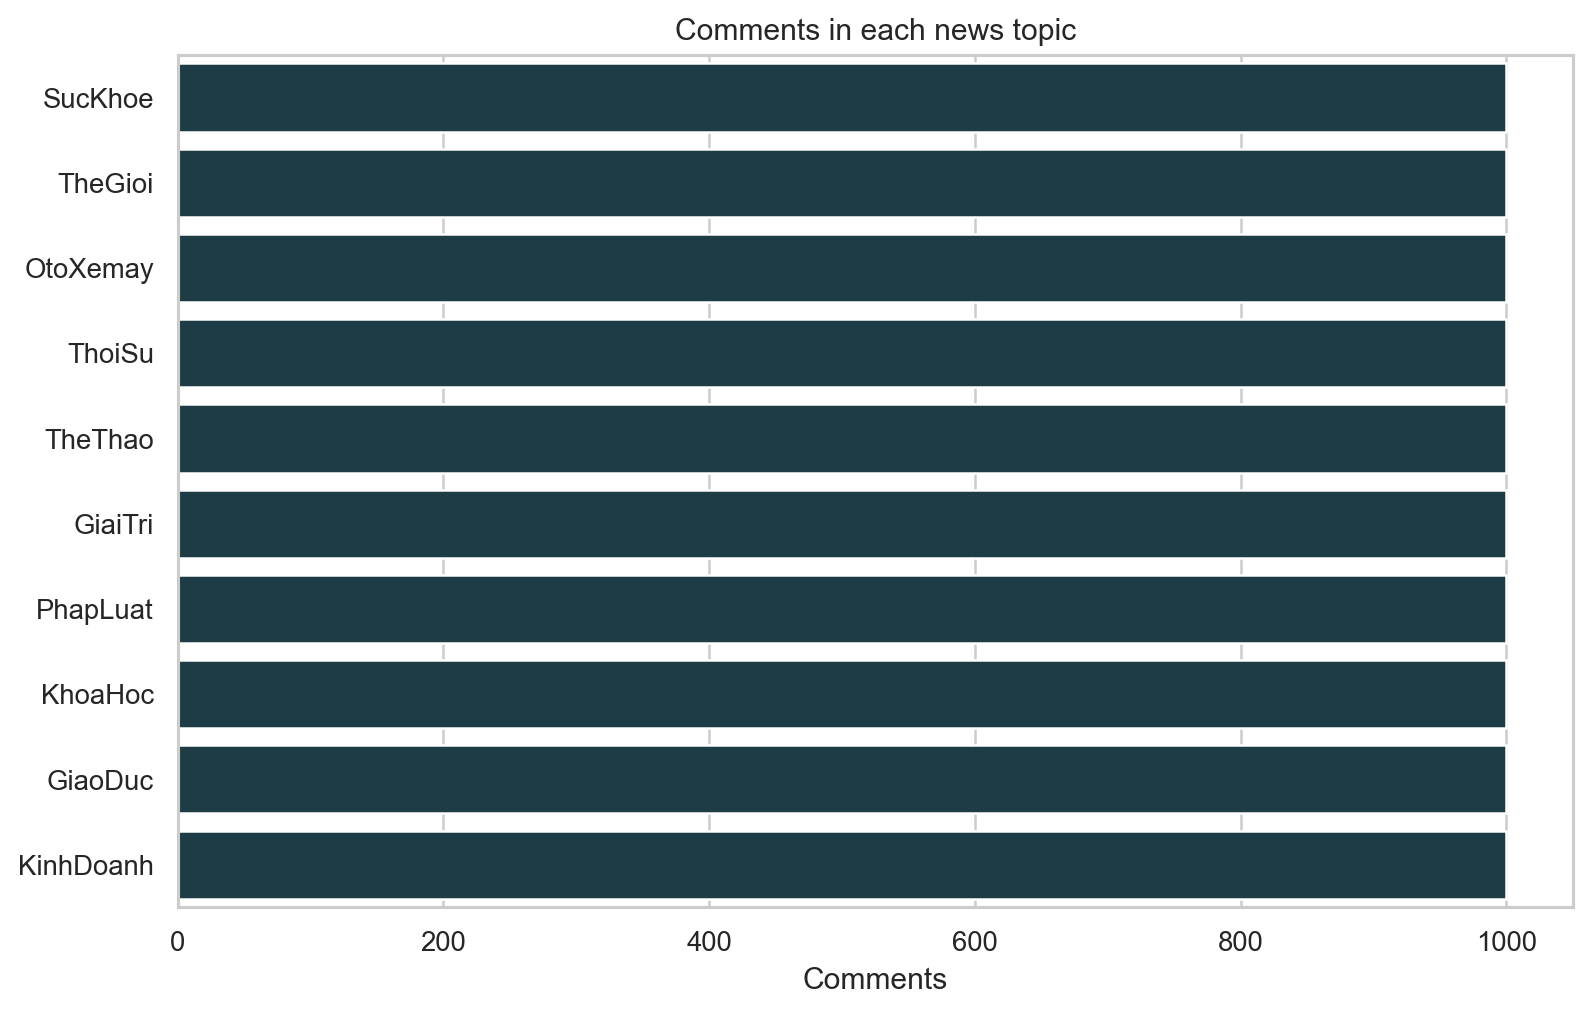
\includegraphics[width=\textwidth]{images/text_03_topic_distribution.png}\\
\small (a) Comments per topic
\end{minipage}\hfill
\begin{minipage}{0.47\textwidth}
\centering
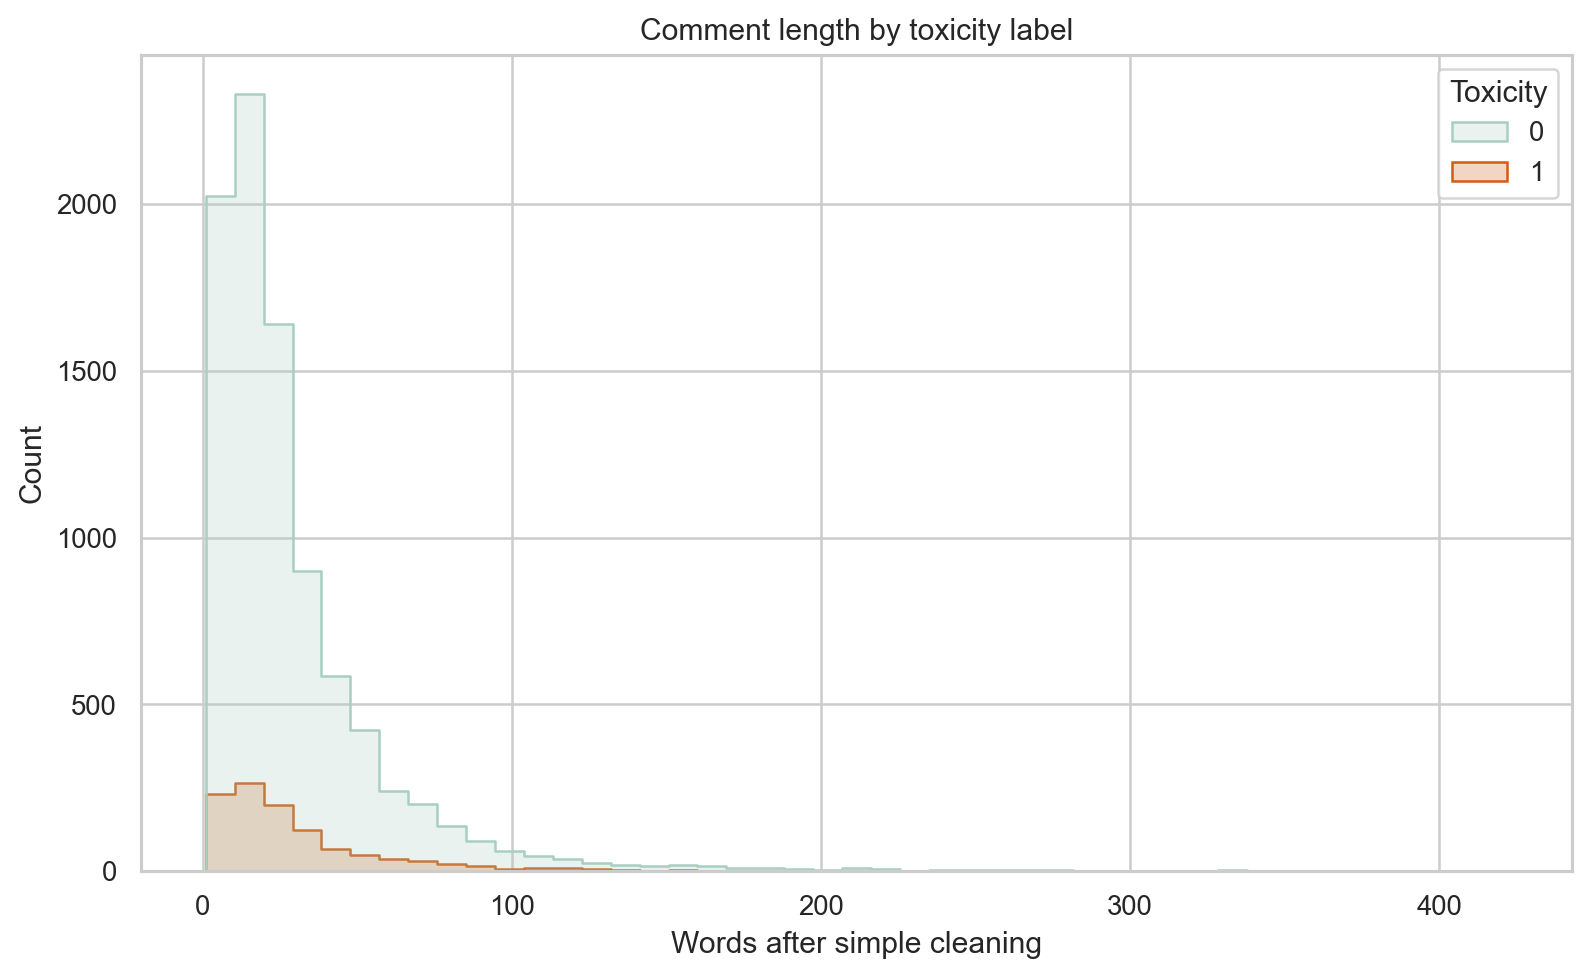
\includegraphics[width=\textwidth]{images/text_04_comment_length.png}\\
\small (b) Comment length after cleaning
\end{minipage}
\caption{Text EDA. The data is balanced by topic, but comment length is right-skewed.}
\label{fig:text-eda}
\end{figure}

The comment-length histogram is right-skewed. Most comments are short, while a small number contain many more characters. The report does not remove long comments or force every comment to the same length. TF-IDF can work with comments of different lengths. The plot is used to understand the data and to remind us that very long comments may contain context that a simple word-and-phrase model cannot fully understand.

\subsection{Text Preparation and Leakage Control}

\subsubsection{Simple Normalization}

The cleaning process is intentionally simple: lowercase text, remove URLs, remove punctuation, and collapse repeated spaces. It is enough to make a first TF-IDF baseline reproducible. It is not intended to solve Vietnamese word segmentation or understand sarcasm.

The steps have direct purposes. Lowercasing treats two words that differ only by capital letters as the same word. Removing a URL avoids giving a unique web address an unnecessary feature. Removing punctuation and repeated spaces creates a consistent text form for counting words and phrases. Vietnamese letters and accents are kept. The report does not apply stemming, manual dictionaries, or a complex tokenizer, because the goal is a small baseline whose operations can be read directly from the notebook.

\begin{lstlisting}[language=Python,caption={Simple preprocessing used in the text notebook.}]
def clean_text(text):
    text = str(text).lower()
    text = re.sub(r"https?://\S+|www\.\S+", " ", text)
    text = re.sub(r"[^\w\s]", " ", text)
    return re.sub(r"\s+", " ", text).strip()
\end{lstlisting}

\subsubsection{Duplicate and Split-Overlap Check}

After this normalization, duplicate comments are checked across the official splits. Thirty-two validation rows and fifteen test rows have normalized text that already appears in training. These rows are excluded from evaluation to avoid direct text leakage. The final validation set has 1,968 rows and the final test set has 985 rows. Training remains at 7,000 rows.

An exact duplicate means that the original comment text is identical. A normalized duplicate may be written with different capital letters, punctuation, or extra spaces, but becomes the same after the simple cleaning function. The normalized check is stricter and is therefore the useful one for a TF-IDF model. Only evaluation rows that overlap with training are removed; the training split is not changed. Consequently, every validation and test score reported below refers to the filtered split of 1,968 or 985 comments, not to the unfiltered official count.

\begin{importantbox}
\textbf{Why this check matters.} If the same sentence occurs in both training and testing, a bag-of-words model can receive credit for memorizing the sentence. Excluding overlap rows does not make the dataset perfect, but it avoids this direct and visible form of leakage.
\end{importantbox}

\subsection{Feature Representation}

\subsubsection{Word and Character TF-IDF}

Two representations are tested. Word TF-IDF uses one-word and two-word phrases, with at most 8,000 features. Character TF-IDF uses character sequences of length three to five, with at most 12,000 features. Logistic Regression is used with balanced class weights for both representations.

TF-IDF changes each comment into a sparse row of numbers. A word or phrase receives a larger value when it is important in one comment but not common in all comments. Thus, a very frequent general word has less influence than a phrase that helps distinguish the two classes. The word model can learn separate signals from words and two-word phrases. The character model uses short sequences of characters instead; it may recognize related spellings or informal variants, but it can also be harder to interpret.

The vectorizers are fitted on training comments only. Terms that appear in validation or test data do not change the vocabulary or the TF-IDF weights learned from training. The word vectorizer ignores terms that occur in only one training comment and uses a maximum of 8,000 features. The character vectorizer uses the same simple rule with a maximum of 12,000 features. These limits keep the experiment small enough to run and inspect without hiding the main idea behind a very large feature space.

\begin{figure}[H]
\centering
\begin{minipage}{0.47\textwidth}
\centering
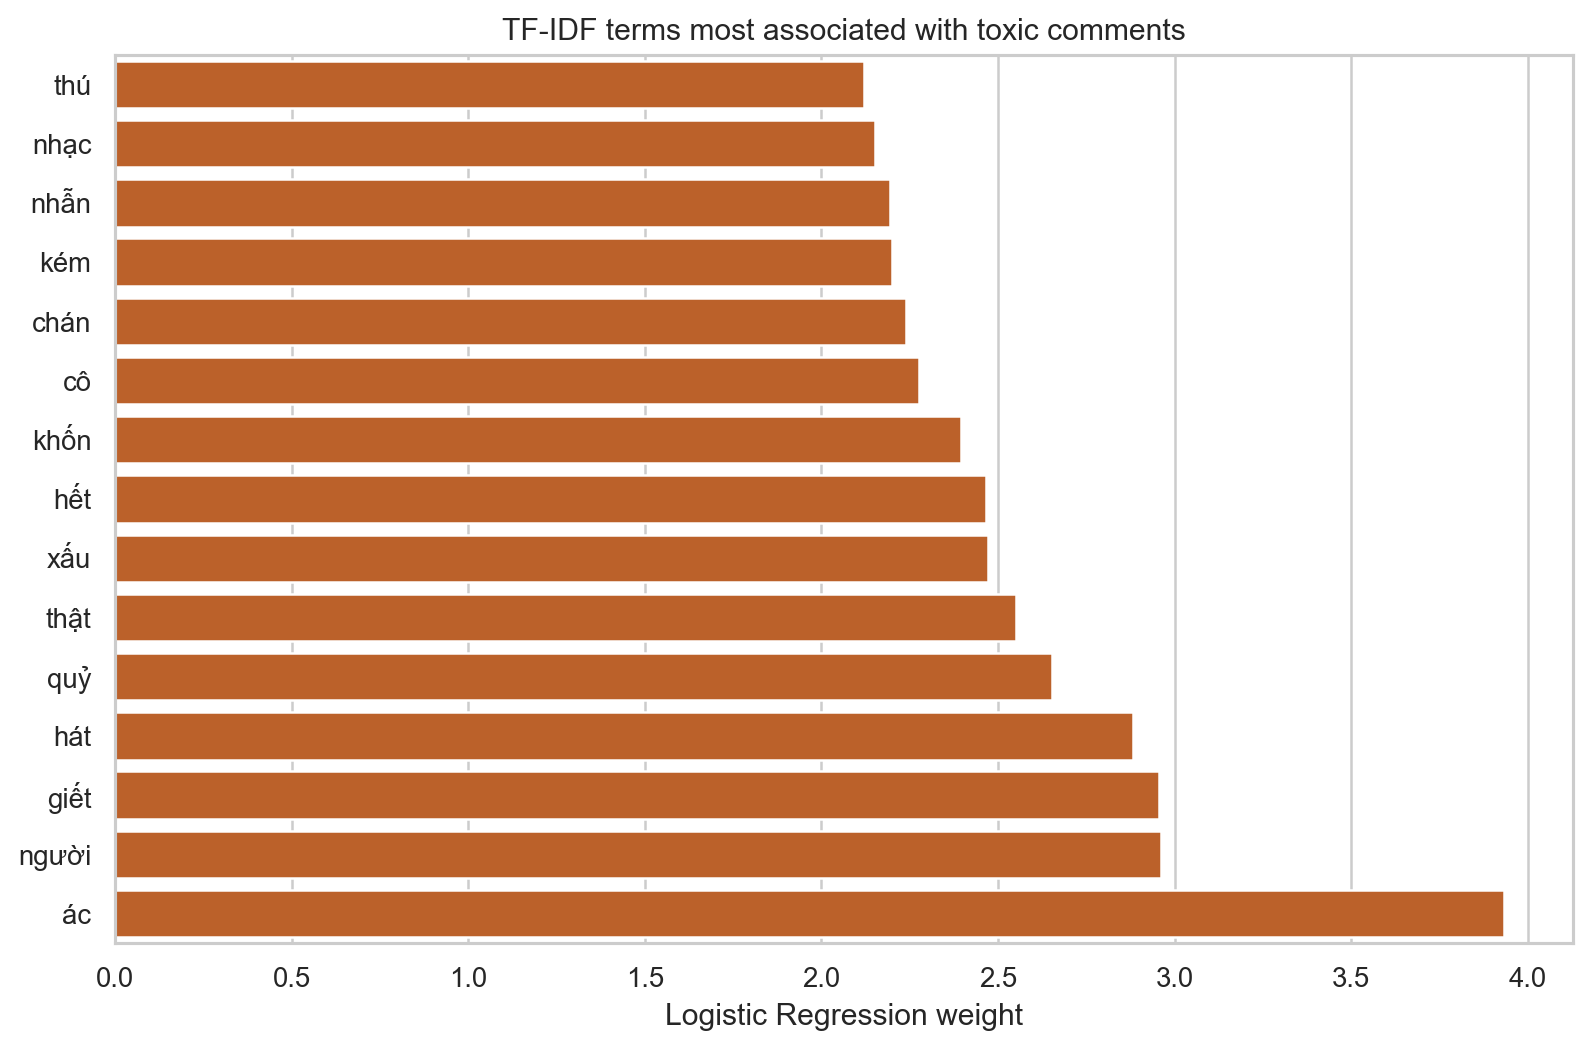
\includegraphics[width=\textwidth]{images/text_05_top_toxic_ngrams.png}\\
\small (a) Higher toxicity weights
\end{minipage}\hfill
\begin{minipage}{0.47\textwidth}
\centering
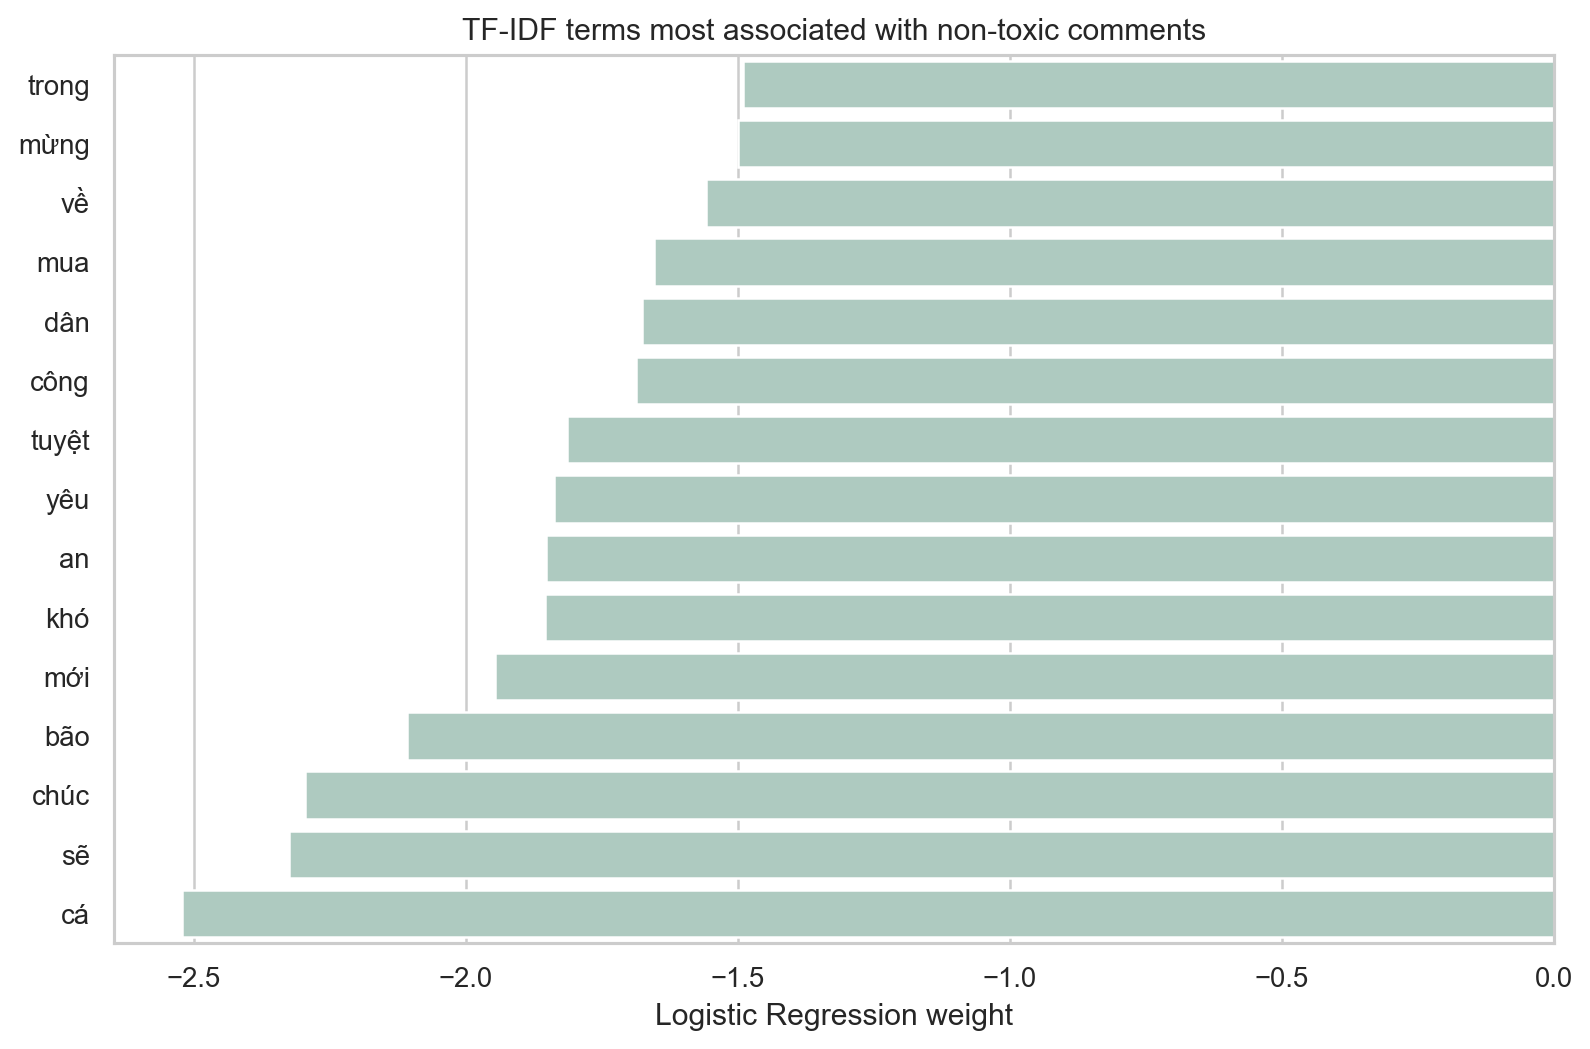
\includegraphics[width=\textwidth]{images/text_06_top_safe_ngrams.png}\\
\small (b) Higher non-toxic weights
\end{minipage}
\caption{Word and phrase weights from the word-level Logistic Regression model. They are model signals, not fixed moderation rules.}
\label{fig:text-ngrams}
\end{figure}

Logistic Regression learns one coefficient for each TF-IDF feature. A feature with a higher positive coefficient pushes a comment towards the toxic class; a feature with a higher negative coefficient pushes it towards the non-toxic class. Figure~\ref{fig:text-ngrams} shows selected high-weight words and phrases. They must not be read as a fixed list of banned or safe expressions. The meaning of a phrase depends on its surrounding words, and a simple linear model sees only the features available in its input vector.

\subsection{Toxicity Model Comparison}

\subsubsection{Validation Models and Selection}

Three simple models are evaluated on the filtered validation set: Multinomial Naive Bayes with word TF-IDF, word TF-IDF with Logistic Regression, and character TF-IDF with Logistic Regression.

Multinomial Naive Bayes is a small baseline that estimates class evidence from feature frequencies and makes a simplifying independence assumption between features. Word TF-IDF plus Logistic Regression learns a direct linear decision from words and two-word phrases. Character TF-IDF plus Logistic Regression uses the same classifier but gives it character fragments instead of word features. For the two Logistic Regression models, balanced class weights increase the cost of mistakes on the less common toxic class. They do not duplicate comments; they only change how the training loss treats the two classes.

\begin{table}[H]
\centering
\caption{Toxicity validation results.}
\label{tab:text-validation}
\begin{tabular}{lrrrr}
\toprule
\textbf{Model} & \textbf{Accuracy} & \textbf{Balanced acc.} & \textbf{F1 toxic} & \textbf{Macro F1} \\
\midrule
Naive Bayes & \textbf{0.884} & 0.506 & 0.026 & 0.482 \\
Word TF-IDF + Logistic & 0.838 & 0.718 & \textbf{0.449} & \textbf{0.677} \\
Char TF-IDF + Logistic & 0.805 & \textbf{0.719} & 0.423 & 0.653 \\
\bottomrule
\end{tabular}
\end{table}

\begin{figure}[H]
\centering
\begin{minipage}{0.56\textwidth}
\centering
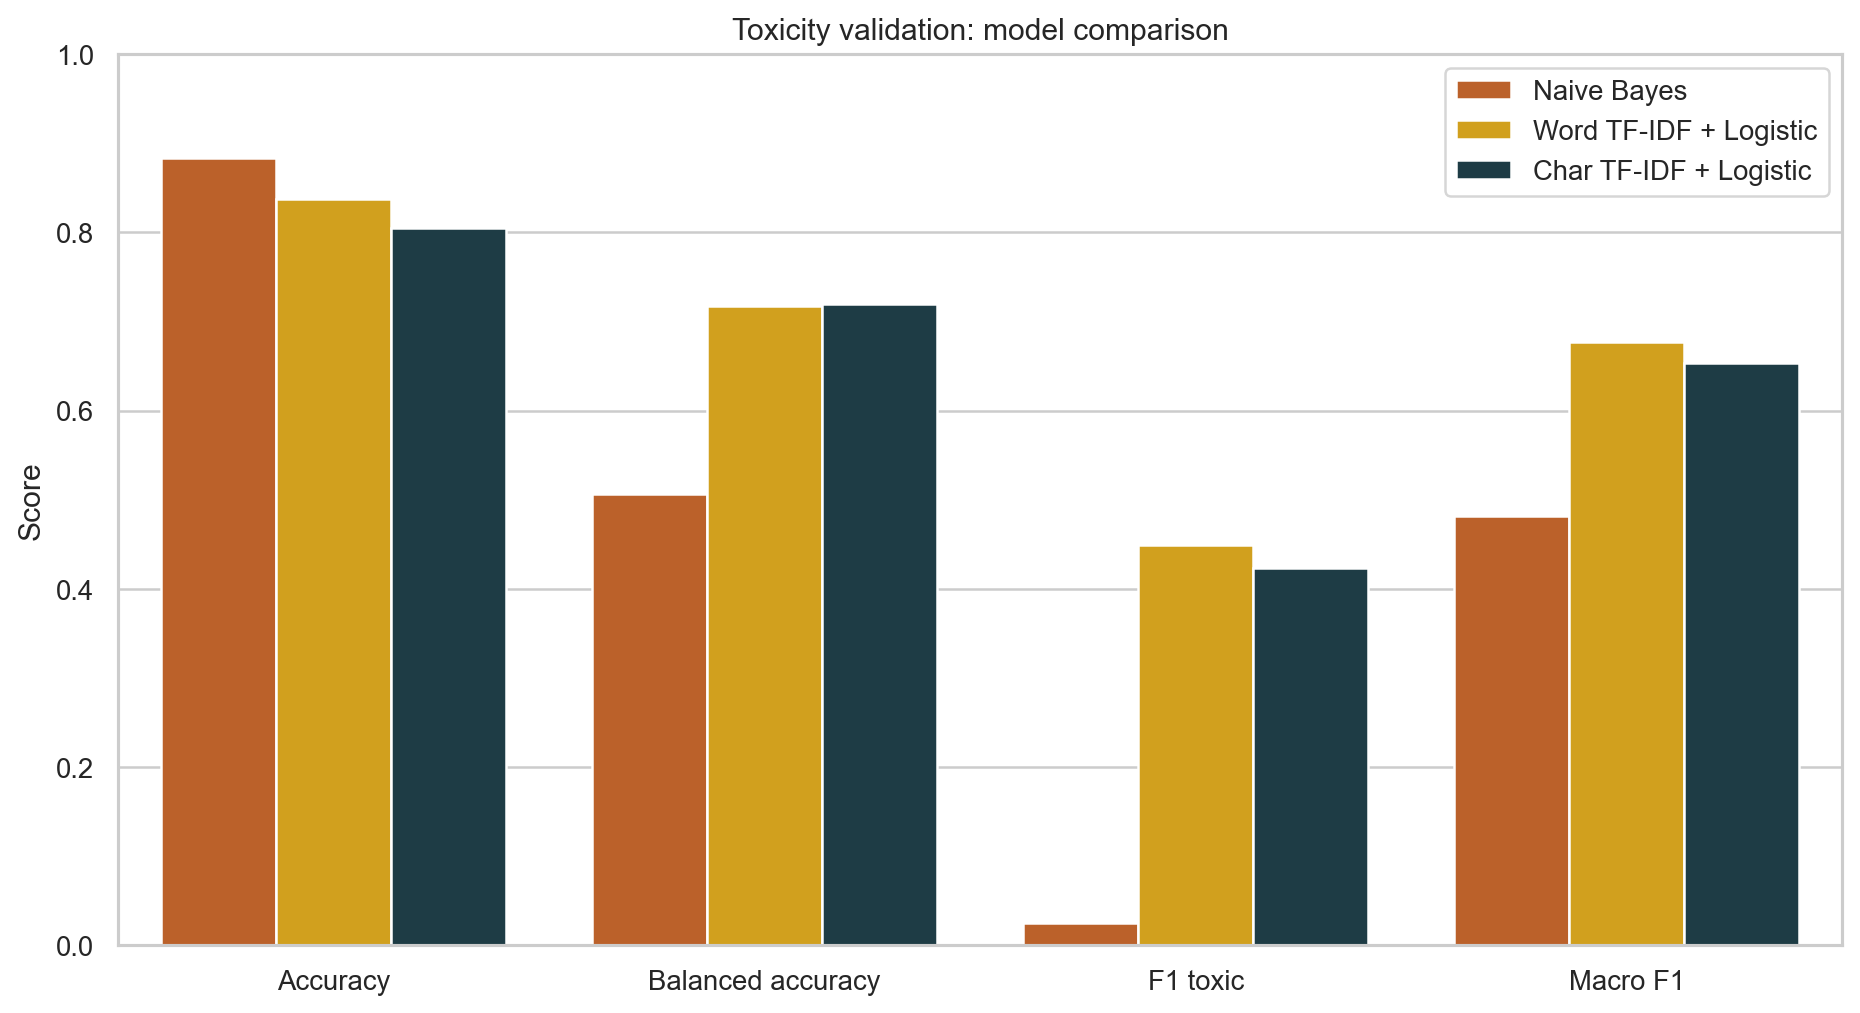
\includegraphics[width=\textwidth]{images/text_07_toxic_model_comparison.png}\\
\small (a) Three-model comparison
\end{minipage}\hfill
\begin{minipage}{0.40\textwidth}
\centering
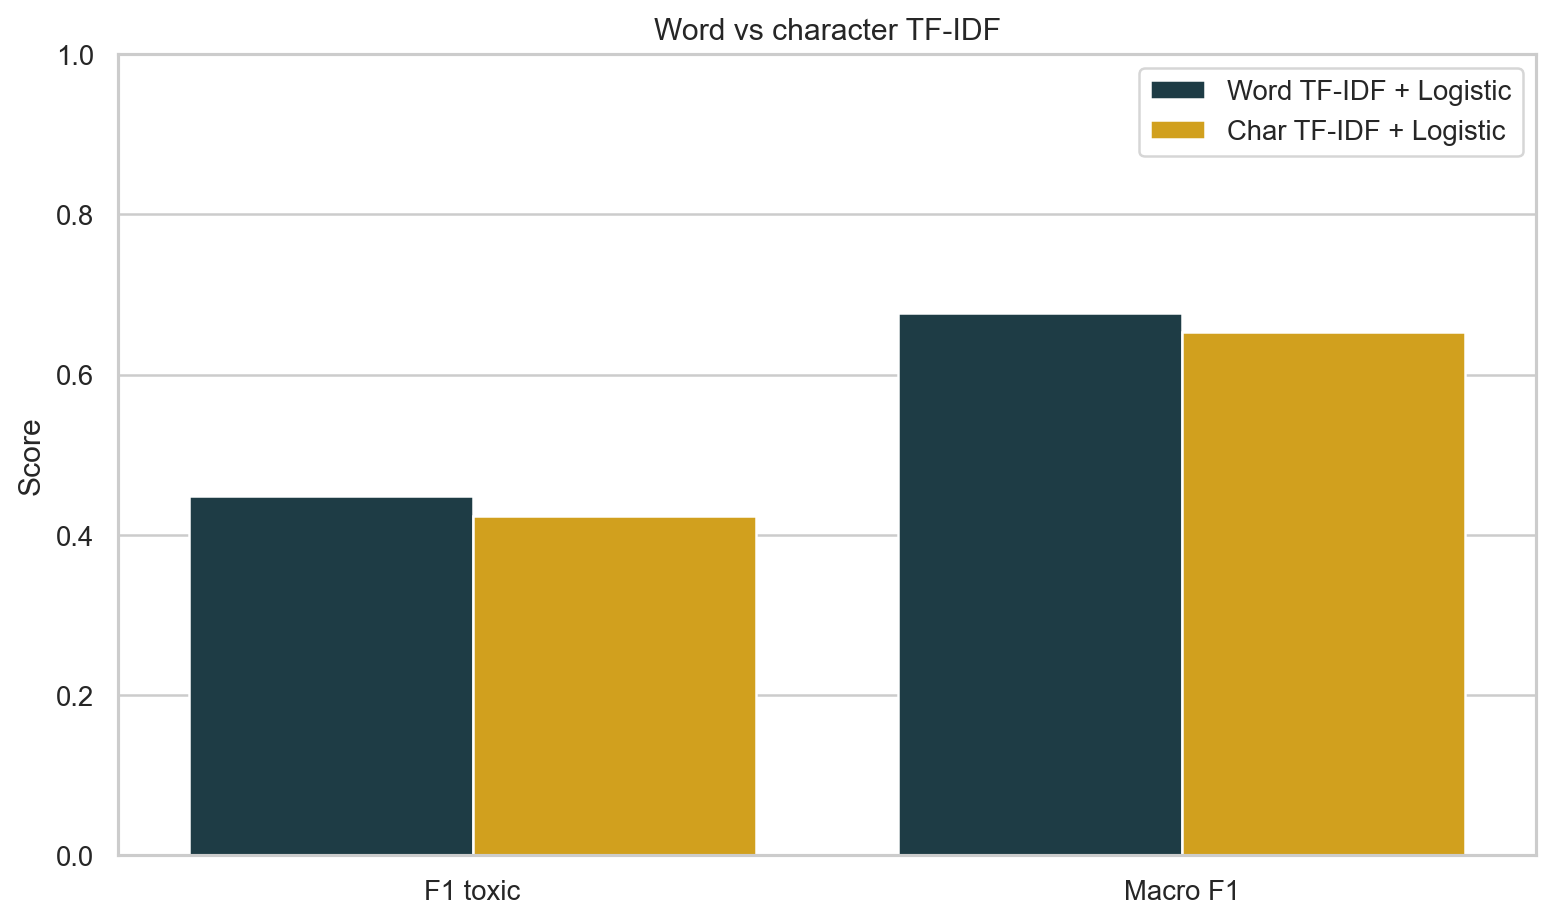
\includegraphics[width=\textwidth]{images/text_08_word_char_comparison.png}\\
\small (b) Word versus character TF-IDF
\end{minipage}
\caption{Validation model comparisons for the toxicity task.}
\label{fig:text-models}
\end{figure}

Naive Bayes has the highest accuracy, but it almost never identifies toxic comments. Its toxic F1 is only 0.026. This is the direct effect of the minority class: a model can receive many correct non-toxic predictions while failing on the comments that need the most attention.

The selected model is word TF-IDF plus Logistic Regression because it has the best macro F1 and toxic F1 on validation. Macro F1 gives the toxic and non-toxic classes the same weight, while toxic F1 focuses specifically on the minority class. Its lower accuracy than Naive Bayes is therefore not a worse practical result. It is a more balanced result: the selected model accepts a small reduction in majority-class accuracy in order to recover many more toxic comments.

\subsection{Final Test Results and Error Review}

\subsubsection{Test Metrics and Confusion Matrices}

The selected toxicity model is tested once on the filtered test split. It achieves 0.842 accuracy, 0.732 balanced accuracy, 0.451 toxic F1, and 0.679 macro F1. The Constructiveness model uses the same word TF-IDF representation and reaches 0.800 macro F1 on the test split.

The confusion matrices in Figure~\ref{fig:text-final} are normalized by true class. Each row represents comments with the same true label, and each cell shows the proportion predicted as each class. The diagonal cells are correct predictions. In the toxicity matrix, the toxic row is the most important row to inspect because it shows how many toxic comments are actually found. The same row-by-row reading applies to constructiveness.

Importantly, the two final macro F1 values should not be compared as if they measured one identical task. Toxicity and constructiveness use different target labels and have different class balances. The purpose of the table is to report how each selected simple model behaves on its own task, not to claim that one social-media property is inherently easier than the other.

\begin{figure}[H]
\centering
\begin{minipage}{0.47\textwidth}
\centering
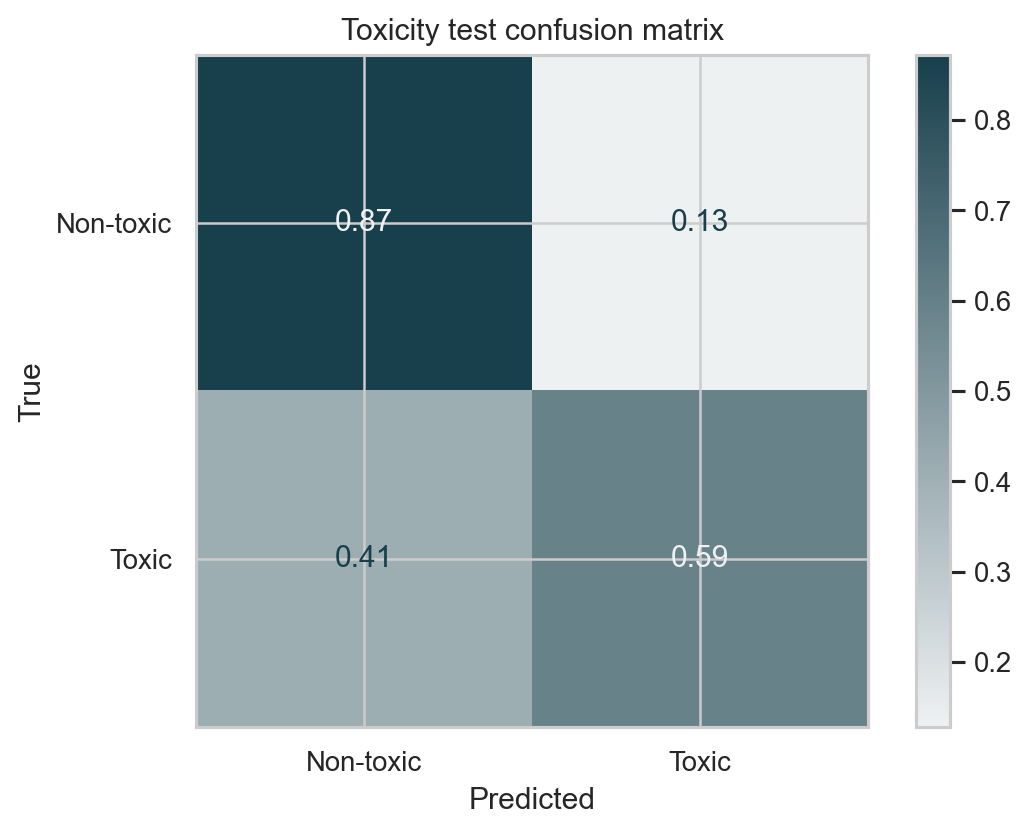
\includegraphics[width=\textwidth]{images/text_09_toxic_confusion_matrix.png}\\
\small (a) Toxicity
\end{minipage}\hfill
\begin{minipage}{0.47\textwidth}
\centering
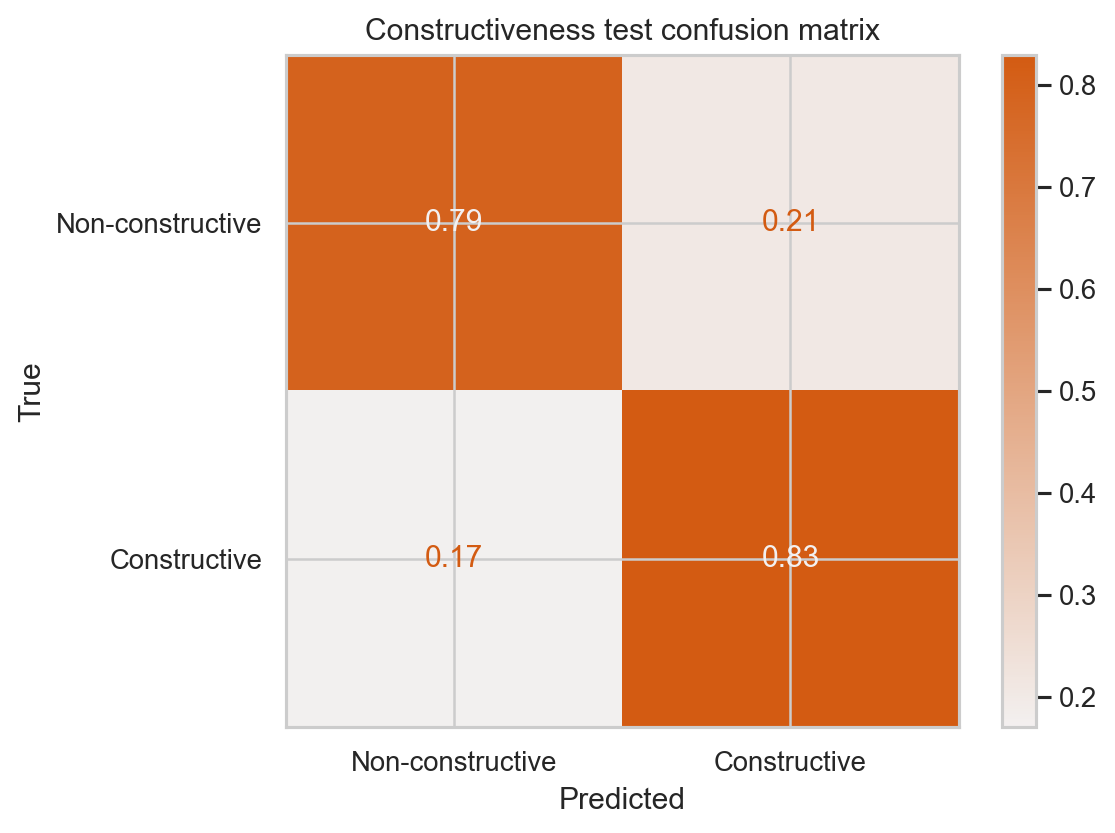
\includegraphics[width=\textwidth]{images/text_10_constructive_confusion_matrix.png}\\
\small (b) Constructiveness
\end{minipage}
\caption{Normalized test confusion matrices for both text tasks.}
\label{fig:text-final}
\end{figure}

\subsubsection{Examples of Classification Errors}

\begin{table}[H]
\centering
\caption{Examples from the first toxicity errors. Text is shortened for readability.}
\label{tab:text-errors}
\small
\begin{tabularx}{\textwidth}{lccX}
\toprule
\textbf{Topic} & \textbf{True} & \textbf{Pred.} & \textbf{Observation} \\
\midrule
OtoXemay & Toxic & Non-toxic & A short sarcastic statement is missed. \\
KhoaHoc & Toxic & Non-toxic & The context is stronger than individual words. \\
PhapLuat & Non-toxic & Toxic & Informal shorthand and strong wording create a false positive. \\
SucKhoe & Non-toxic & Toxic & A long context-dependent sentence is difficult for n-grams. \\
\bottomrule
\end{tabularx}
\end{table}

A false negative occurs when a toxic comment is predicted as non-toxic. This is a missed harmful comment. A false positive occurs when a non-toxic comment is predicted as toxic. This can incorrectly flag a normal comment. The examples show why both error types occur. Sarcasm often has a meaning that is different from its individual words. Informal spelling, shorthand, and a sentence that depends on earlier discussion are also difficult for a model that only observes local words and phrases.

\subsubsection{Key Findings and Limitations}

\begin{importantbox}
\textbf{Text conclusion.} Word TF-IDF plus balanced Logistic Regression is a suitable simple baseline for this dataset. It is easy to inspect and it is better than the accuracy-only Naive Bayes baseline. Its limits are clear: sarcasm, shorthand, and long contextual comments still cause errors. The model can support review, for example by ordering comments for a moderator to inspect, but should not replace human judgement in moderation.
\end{importantbox}

\clearpage
\section{Image Data: Intel Image Classification}
\label{sec:image}

\subsection{Task Objective and Dataset}

This task classifies a natural scene image into one of six labels: \textit{buildings}, \textit{forest}, \textit{glacier}, \textit{mountain}, \textit{sea}, and \textit{street}. The selected source is the Intel Image Classification dataset on Kaggle \cite{intel}. It contains 17,034 labelled RGB JPEG images. Every original image is 150 by 150 pixels, which is above the course recommendation of a short side of 128 pixels. The dataset has 14,034 images in its source training folder and 3,000 images in a separate source test folder.

The image labels are supplied by the dataset. This project does not claim to discover a new scene category or to judge whether a source label is perfect. Its purpose is to build a clear and reproducible classroom classifier: inspect the images, define a fair split, compare two understandable pretrained approaches, and then measure the selected approach on images that were not used earlier.

\begin{importantbox}
\textbf{Task fit.} The dataset has more than 5,000 images and more than three target classes. It is therefore large enough for the Image-data task, while the six everyday scene classes remain understandable for a first image-classification project.
\end{importantbox}

\subsection{Dataset Structure and Image EDA}

The downloaded dataset has two labelled folders: \texttt{seg\_train} and \texttt{seg\_test}. Each class has its own subfolder, so the parent folder name becomes the target label. The notebook uses \texttt{torchvision.datasets.ImageFolder} to read this simple structure. It does not read a hidden metadata column or a filename-derived target. The class order is alphabetical and is fixed as buildings, forest, glacier, mountain, sea, and street.

Table~\ref{tab:intel-class-counts} shows the source distribution. The class counts are similar but not identical. Glacier has the most source-test images (553), while buildings has the fewest (437). For this reason, ordinary accuracy is reported together with balanced accuracy and macro F1. Macro F1 first computes an F1 score for each class and then gives every class the same weight. This makes a model that only succeeds on a common class less attractive.

\begin{table}[H]
\centering
\caption{Intel Image Classification source folders and labels.}
\label{tab:intel-class-counts}
\begin{tabular}{lrrr}
\toprule
\textbf{Scene class} & \textbf{Source train} & \textbf{Source test} & \textbf{Total} \\
\midrule
Buildings & 2,191 & 437 & 2,628 \\
Forest & 2,271 & 474 & 2,745 \\
Glacier & 2,404 & 553 & 2,957 \\
Mountain & 2,512 & 525 & 3,037 \\
Sea & 2,274 & 510 & 2,784 \\
Street & 2,382 & 501 & 2,883 \\
\midrule
\textbf{Total} & \textbf{14,034} & \textbf{3,000} & \textbf{17,034} \\
\bottomrule
\end{tabular}
\end{table}

Figure~\ref{fig:intel-examples} gives one real image from each label. The examples already explain why this is a useful task: forest is visually distinctive because of repeated green texture, while glacier and mountain can share rocks, snow, and sky. Buildings and street can also share urban structures. These overlaps should appear again in the error analysis rather than being hidden behind a single score.

\begin{figure}[H]
\centering
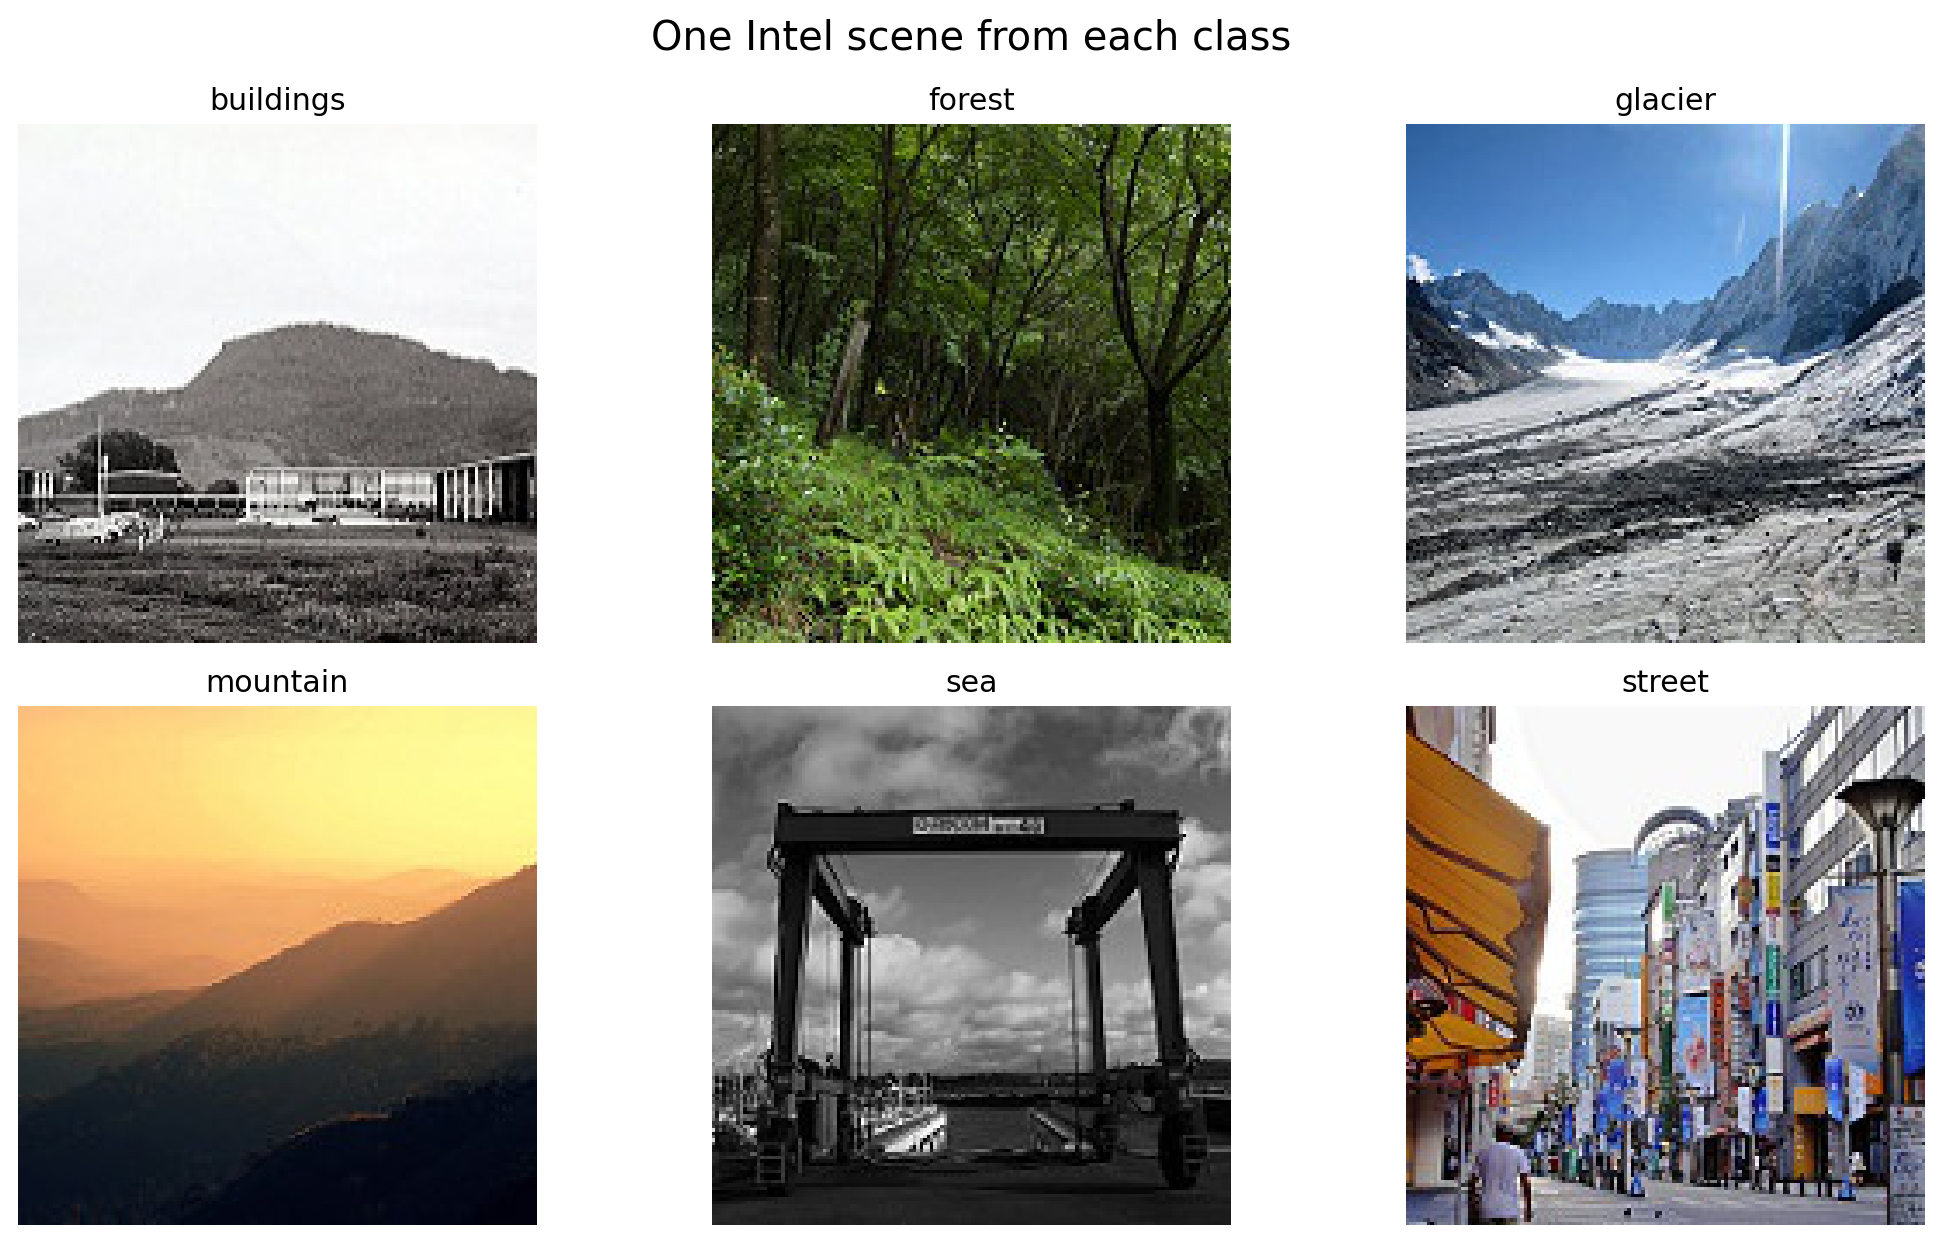
\includegraphics[width=\textwidth]{images/intel_01_scene_examples.png}
\caption{One source image from each Intel scene class.}
\label{fig:intel-examples}
\end{figure}

Figure~\ref{fig:intel-eda} contains two independent EDA plots. The first confirms the per-class counts. The second uses mean pixel brightness as a small quality check. Brightness is not added as a separate model feature. It is only used to show that lighting, snow, clouds, and shadows vary across images, so a consistent image normalization step is necessary before using ImageNet-pretrained weights.

\begin{figure}[H]
\centering
\begin{minipage}{0.52\textwidth}
\centering
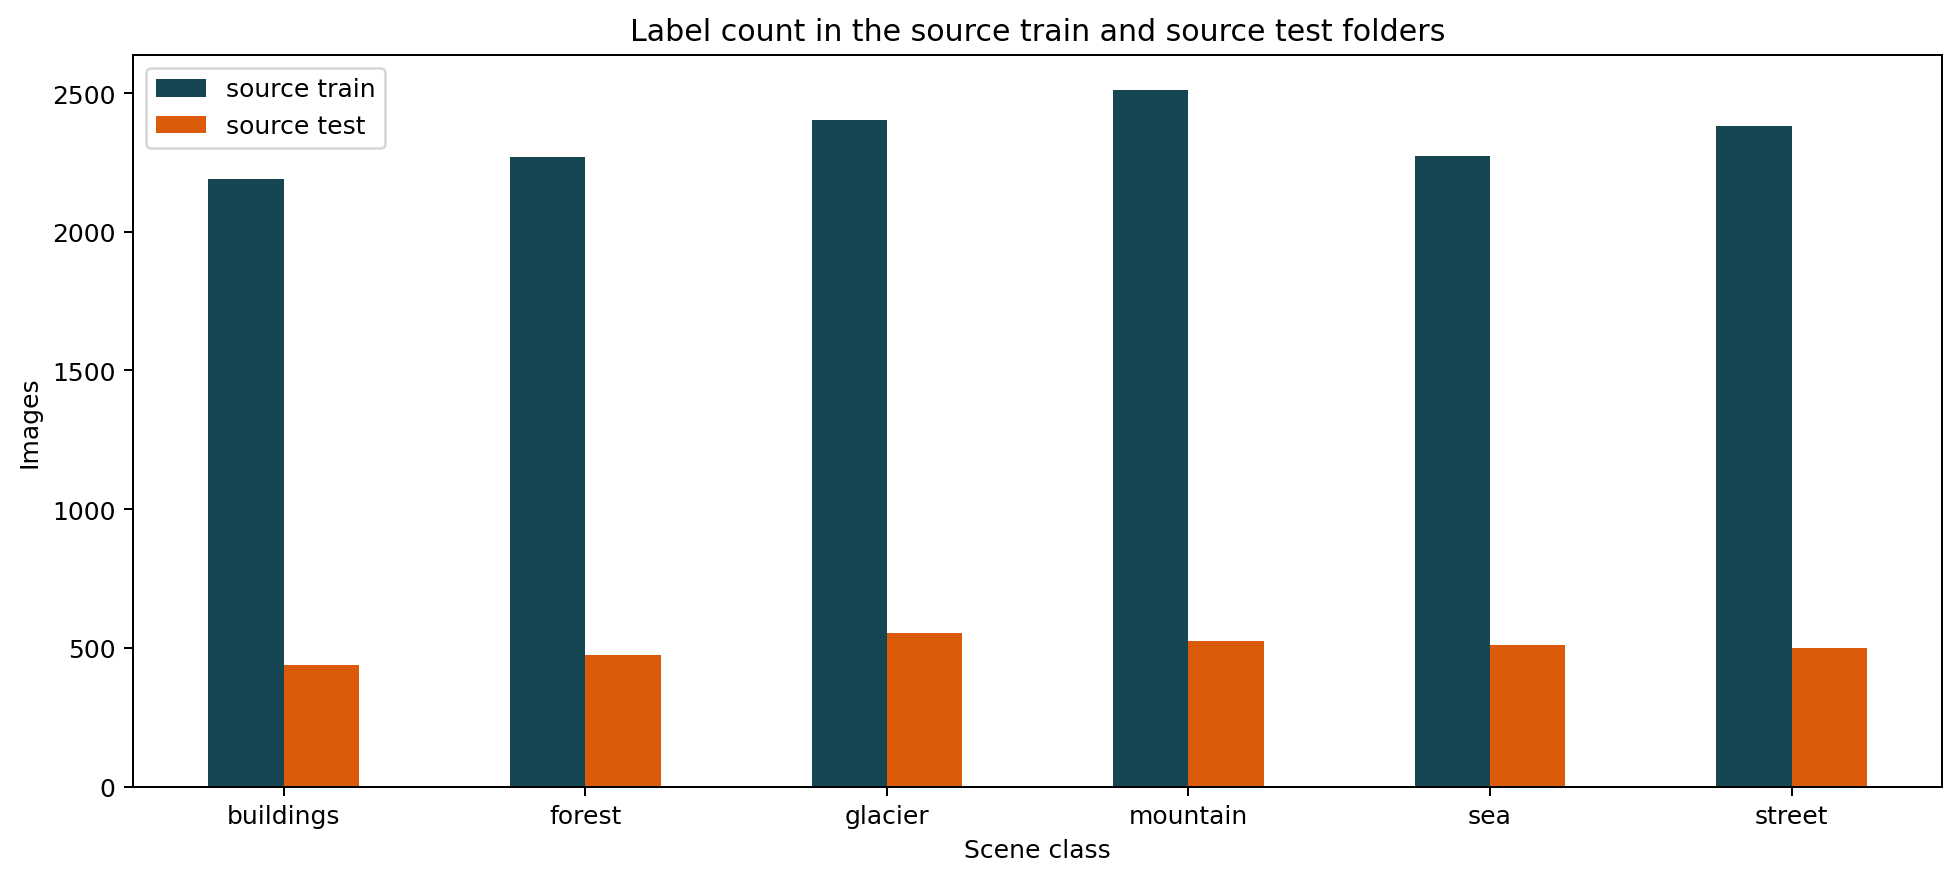
\includegraphics[width=\textwidth]{images/intel_02_class_distribution.png}\\
\small (a) Source class counts
\end{minipage}\hfill
\begin{minipage}{0.42\textwidth}
\centering
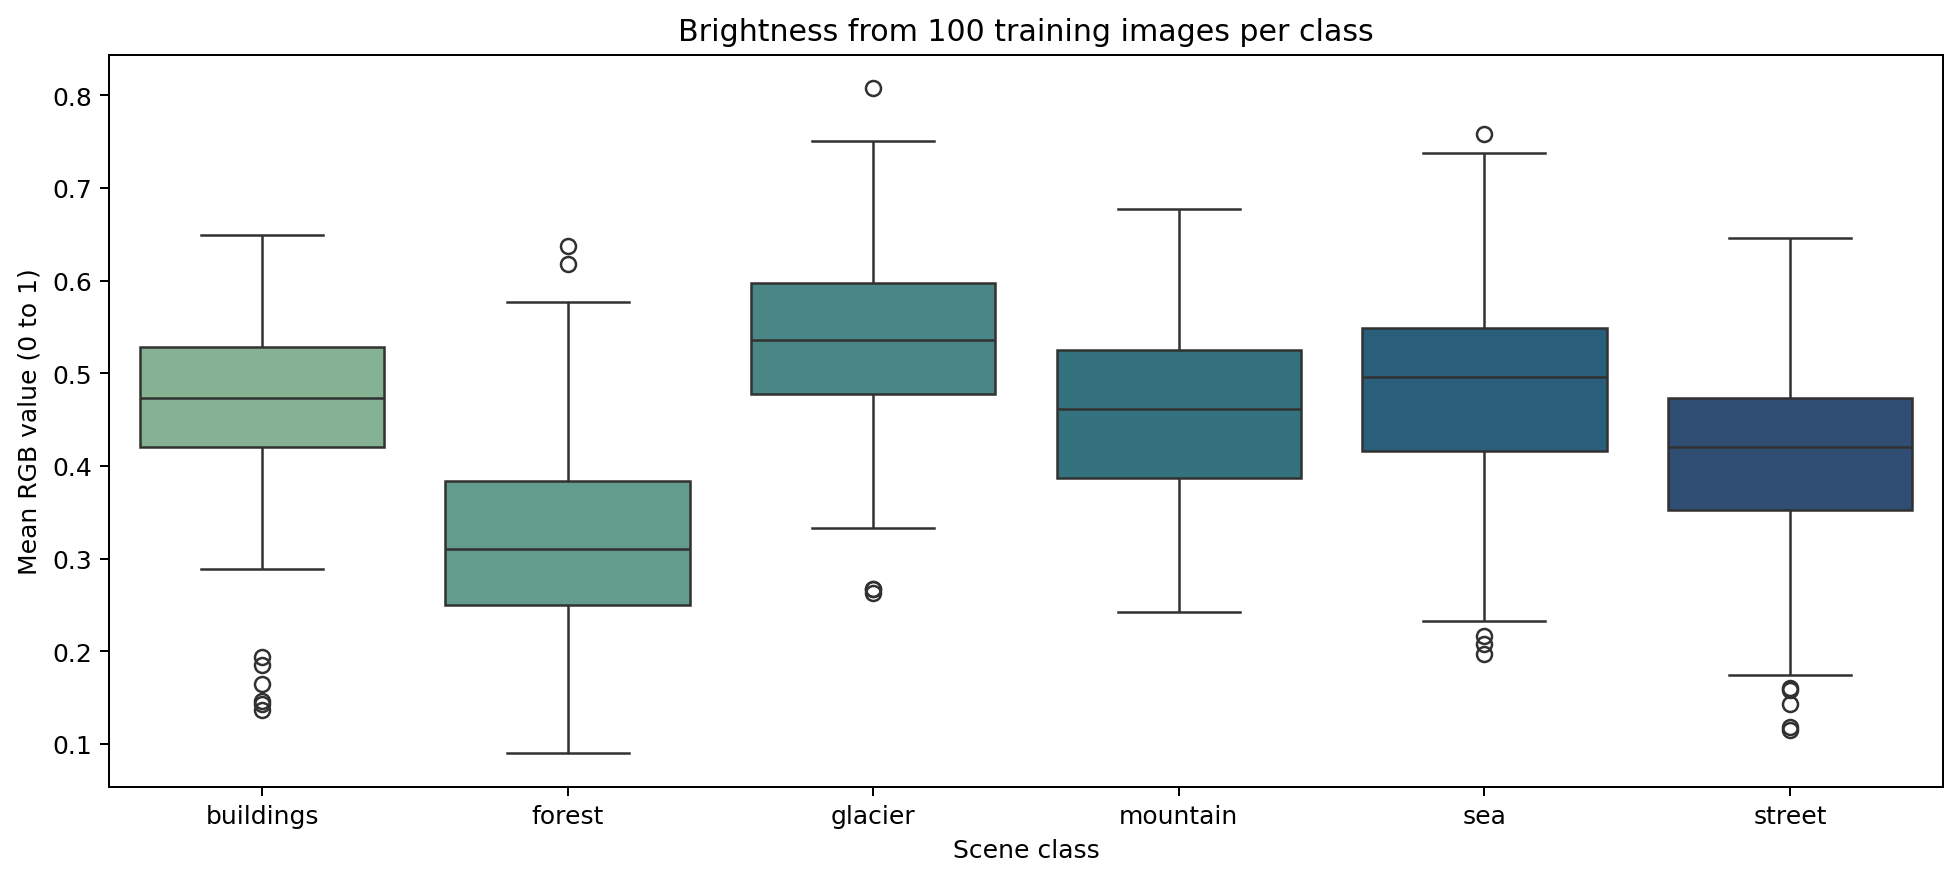
\includegraphics[width=\textwidth]{images/intel_03_brightness_by_class.png}\\
\small (b) Brightness check by class
\end{minipage}
\caption{Simple image EDA. The brightness plot is an inspection result, not an input column.}
\label{fig:intel-eda}
\end{figure}

\subsection{Split, Quality Control, and Leakage Prevention}

The source \texttt{seg\_test} folder is reserved as the final test set from the beginning. It is never used to fit a model, choose an epoch, choose a transform, or compare the two approaches. The source \texttt{seg\_train} folder is split with seed 42 and stratification: 80\% becomes the fitting set and 20\% becomes the validation set. Stratification keeps the six class proportions close to the original source distribution.

\begin{table}[H]
\centering
\caption{Fair split used for the Intel image task.}
\label{tab:intel-split}
\begin{tabular}{lrl}
\toprule
\textbf{Split} & \textbf{Images} & \textbf{Use} \\
\midrule
Training & 11,227 & Fit the Logistic Regression classifier and MobileNetV3 head \\
Validation & 2,807 & Select the final approach using macro F1 \\
Source test & 3,000 & Evaluate the selected approach once at the end \\
\bottomrule
\end{tabular}
\end{table}

The code keeps the source folders separate and uses each image path in only one of these three roles. There is no outcome-like metadata or identifier used as an input: the input is only the RGB image. All 17,034 JPEG files loaded successfully during the executed run. This does not prove that a public dataset has no visually similar pictures, but it prevents the direct leakage that would occur if the provided test folder entered the split or model-selection step.

\subsection{Preprocessing and Augmentation}

MobileNetV3-Small is pretrained on ImageNet. For feature extraction and evaluation, the notebook applies the preprocessing supplied with the pretrained weights: resize, centre crop, tensor conversion, and ImageNet channel normalization. The original data are 150 by 150 pixels; the network receives its standard 224 by 224 view after resizing. This makes the numerical pixel range compatible with the pretrained network.

The training view also uses one simple augmentation: a random horizontal flip. Mirroring a forest, a mountain, or a street does not change its scene label, but it prevents the new classifier head from relying too strongly on a left-right layout. Validation and test images never receive the random flip, so their predictions are repeatable. Figure~\ref{fig:intel-preparation} shows one augmentation example and the five-epoch learning curve.

\begin{figure}[H]
\centering
\begin{minipage}{0.42\textwidth}
\centering
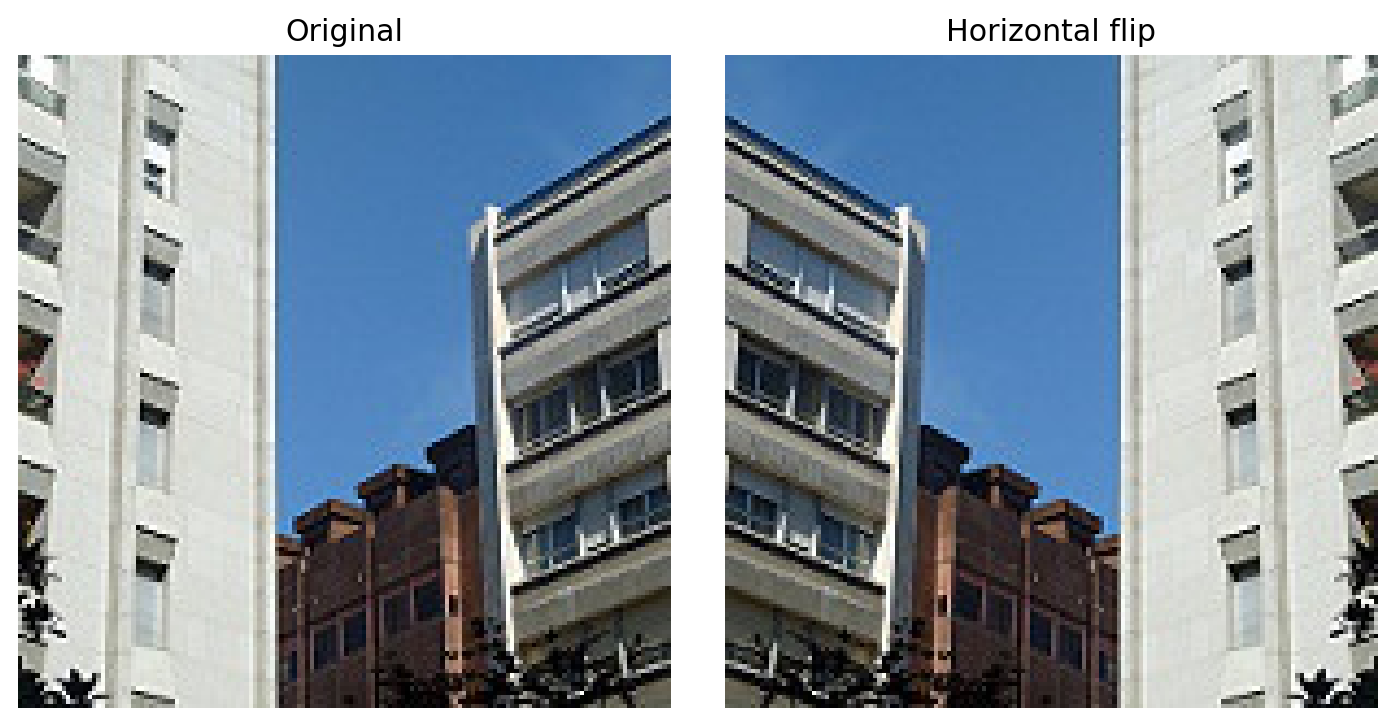
\includegraphics[width=\textwidth]{images/intel_04_augmentation_example.png}\\
\small (a) Random horizontal flip
\end{minipage}\hfill
\begin{minipage}{0.53\textwidth}
\centering
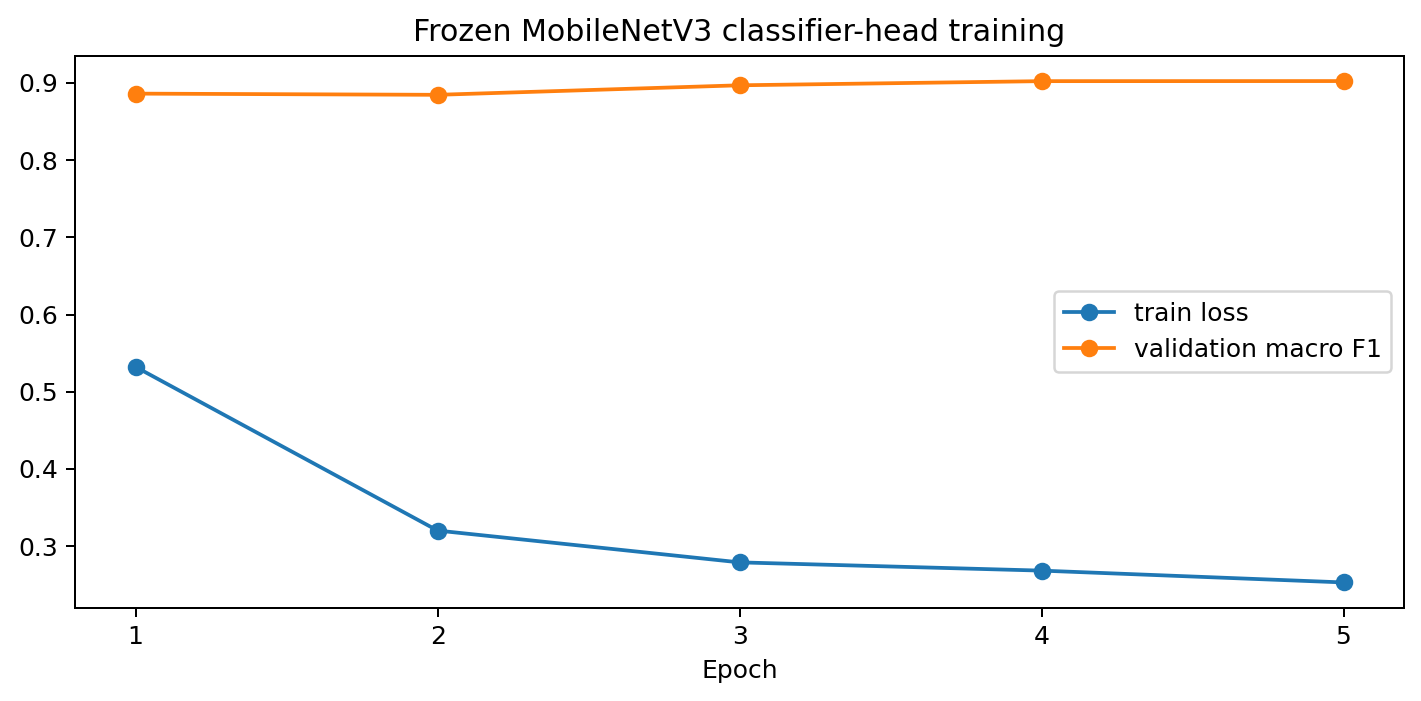
\includegraphics[width=\textwidth]{images/intel_05_training_history.png}\\
\small (b) Frozen-head training history
\end{minipage}
\caption{The only random augmentation and the five-epoch training history.}
\label{fig:intel-preparation}
\end{figure}

\subsection{Model Comparison}

Both candidate models reuse the same pretrained MobileNetV3-Small visual backbone. This meets the deep-learning requirement without asking a beginner to train a convolutional network from scratch. The first model removes the final classifier, so each image becomes a 576-value pretrained feature vector. A balanced Logistic Regression model is then fitted to these vectors. This is a useful simple baseline: the deep network describes visual patterns, and a linear classifier makes the final class decision.

The second model freezes the MobileNetV3 feature layers and replaces its final output layer with a six-class classifier. Only the classifier head is updated for five epochs with Adam, learning rate 0.0003, and class-weighted cross-entropy. This is light transfer learning. It allows the final layer to adapt to the six Intel labels without changing the large pretrained feature extractor.

Table~\ref{tab:intel-validation} compares the models only on validation images. The pretrained-feature Logistic Regression model has the higher validation macro F1 (0.906 versus 0.902), so it is selected before the source-test labels are evaluated. The difference is small, but the selection rule is explicit and does not use the test score.

\begin{table}[H]
\centering
\caption{Validation comparison. Selection is based on macro F1.}
\label{tab:intel-validation}
\begin{tabular}{lrrr}
\toprule
\textbf{Model} & \textbf{Accuracy} & \textbf{Balanced acc.} & \textbf{Macro F1} \\
\midrule
Pretrained features + Logistic Regression & \textbf{0.904} & \textbf{0.906} & \textbf{0.906} \\
Frozen MobileNetV3 head & 0.900 & 0.902 & 0.902 \\
\bottomrule
\end{tabular}
\end{table}

\begin{figure}[H]
\centering
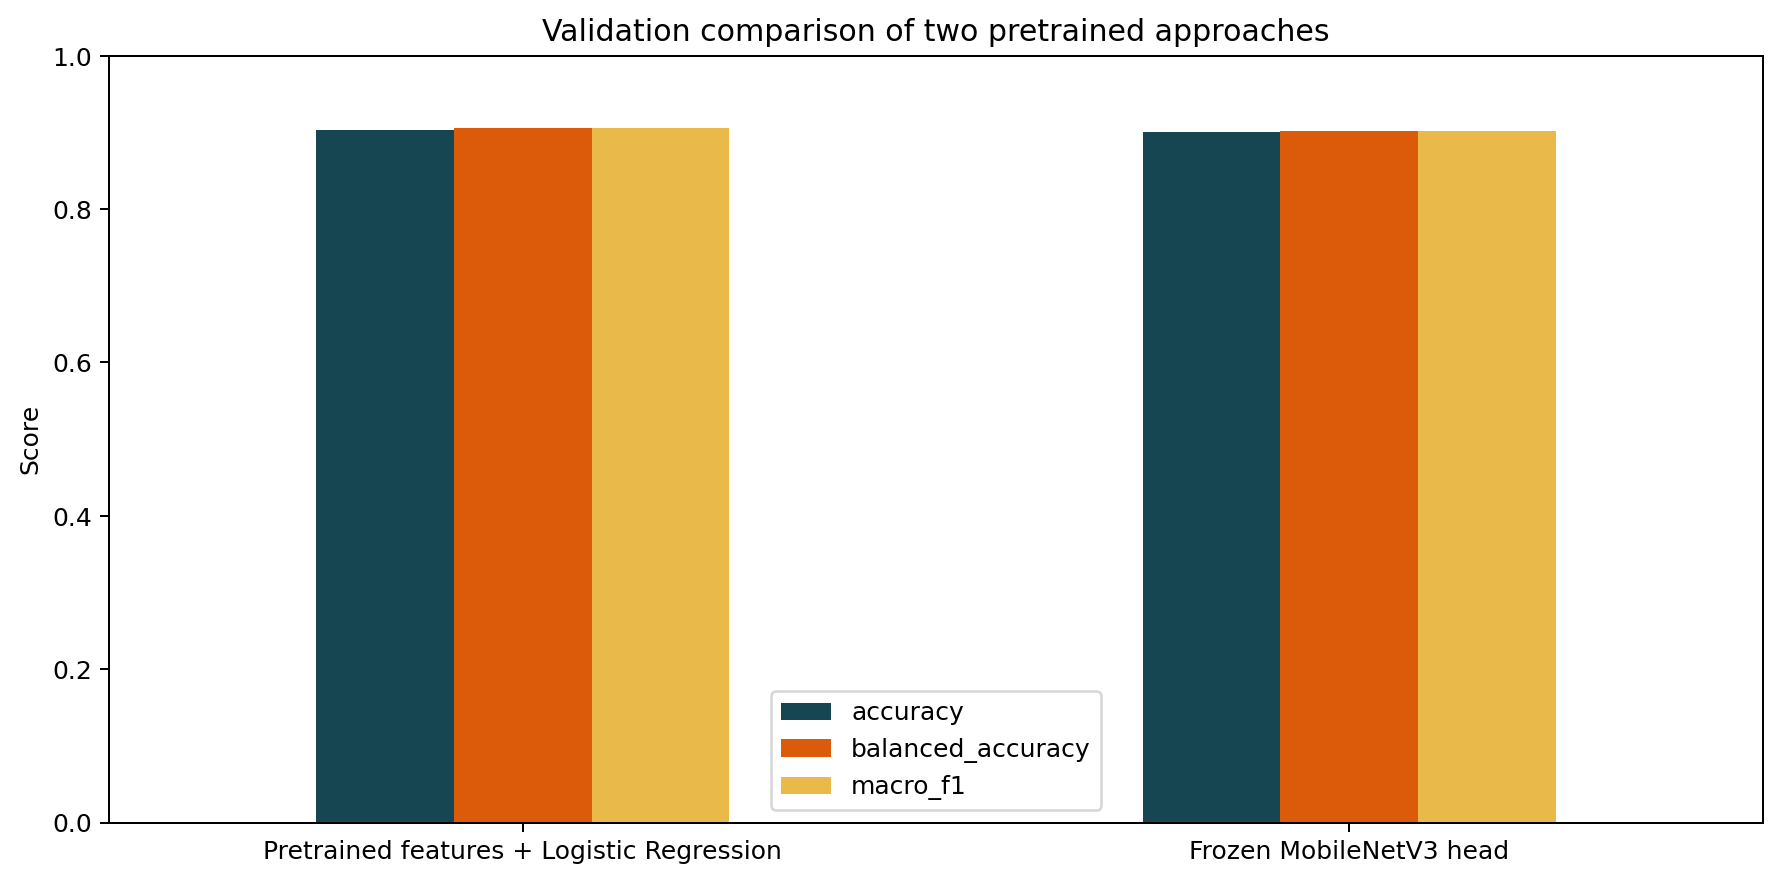
\includegraphics[width=0.80\textwidth]{images/intel_06_model_comparison.png}
\caption{Validation scores for the two pretrained approaches.}
\label{fig:intel-models}
\end{figure}

\subsection{Final Test Evaluation and Error Review}

The selected pretrained-feature Logistic Regression model is evaluated once on the untouched source test folder. It obtains accuracy 0.914, balanced accuracy 0.916, and macro F1 0.916. The close values show that the result is not caused only by one large class. Forest is the easiest class (F1 0.994), while glacier and mountain are harder (F1 0.860 and 0.863). This matches the visual overlap seen in the example images.

\begin{table}[H]
\centering
\caption{Per-class result of the selected model on the 3,000-image source test set.}
\label{tab:intel-test}
\begin{tabular}{lrrr}
\toprule
\textbf{Class} & \textbf{Precision} & \textbf{Recall} & \textbf{F1} \\
\midrule
Buildings & 0.903 & 0.920 & 0.912 \\
Forest & 0.996 & 0.992 & 0.994 \\
Glacier & 0.863 & 0.857 & 0.860 \\
Mountain & 0.867 & 0.859 & 0.863 \\
Sea & 0.938 & 0.949 & 0.943 \\
Street & 0.928 & 0.922 & 0.925 \\
\midrule
\textbf{Macro average} & \textbf{0.916} & \textbf{0.916} & \textbf{0.916} \\
\bottomrule
\end{tabular}
\end{table}

Figure~\ref{fig:intel-confusion} is normalized row by row. A diagonal cell is the recall for one true class. The darker diagonal cells confirm good recognition of forest and sea. The main visible confusion is between glacier and mountain, which is expected because both can contain rock, snow, cloud, and a distant horizon.

\begin{figure}[H]
\centering
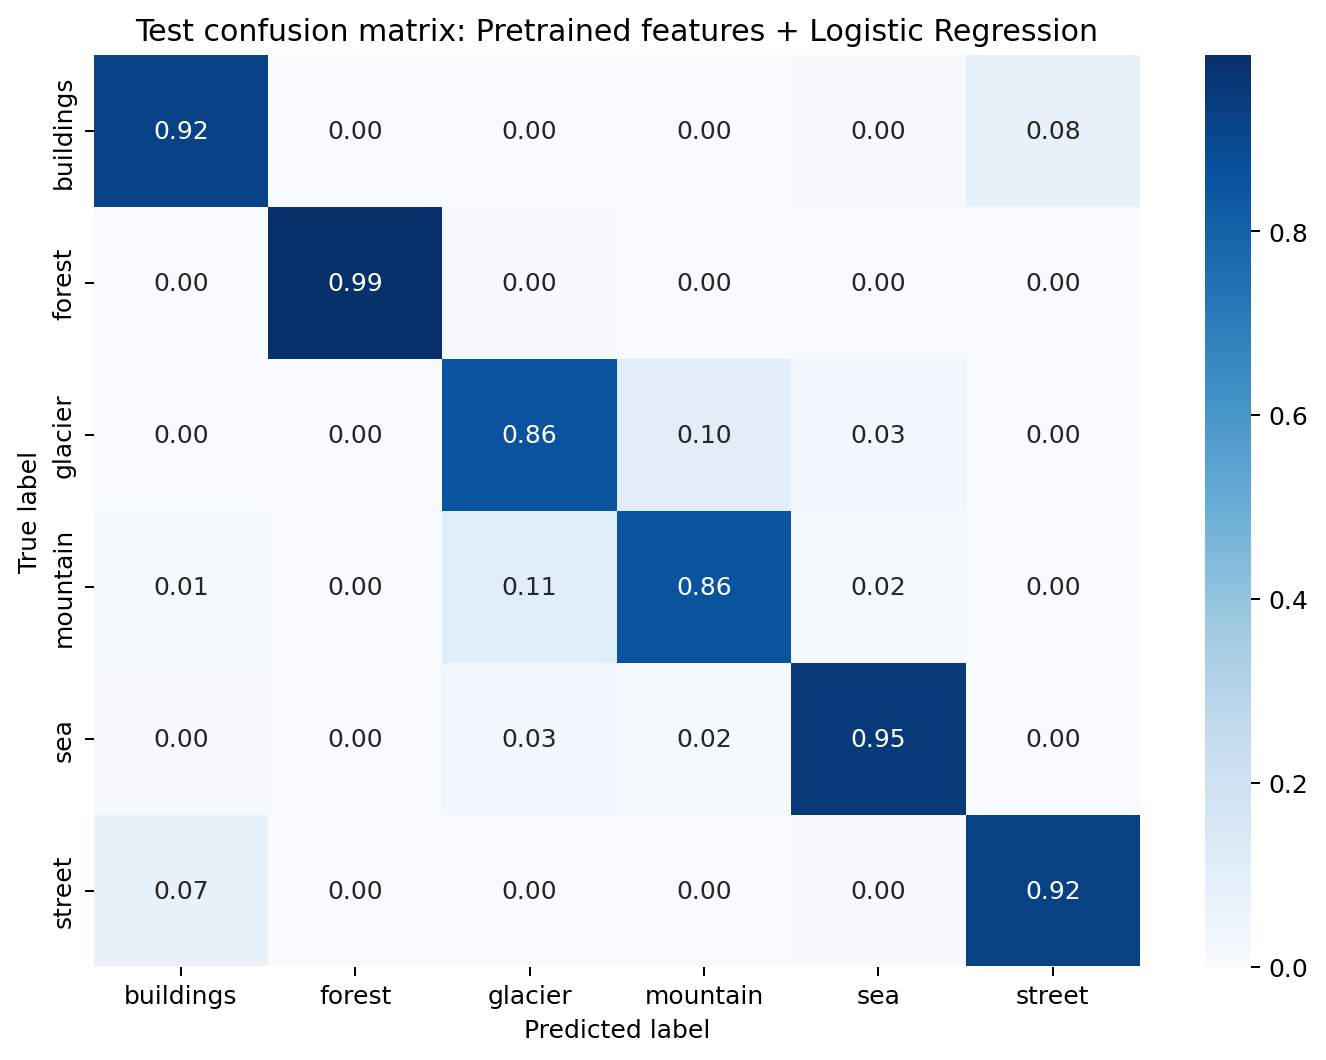
\includegraphics[width=0.90\textwidth]{images/intel_07_confusion_matrix.png}
\caption{Normalized source-test confusion matrix for the selected model.}
\label{fig:intel-confusion}
\end{figure}

There are 257 wrong predictions among the 3,000 test images. The two most frequent directional errors are glacier predicted as mountain (58 images) and mountain predicted as glacier (58 images). Street predicted as buildings (35 images) and buildings predicted as street (33 images) are the next important pair. Figure~\ref{fig:intel-errors} shows twelve concrete mistakes. These examples are more useful than claiming that a 0.916 macro F1 is perfect: scene boundaries can be visually ambiguous, and a model can fail on unusual lighting, distant objects, or mixed scenery.

\begin{figure}[H]
\centering
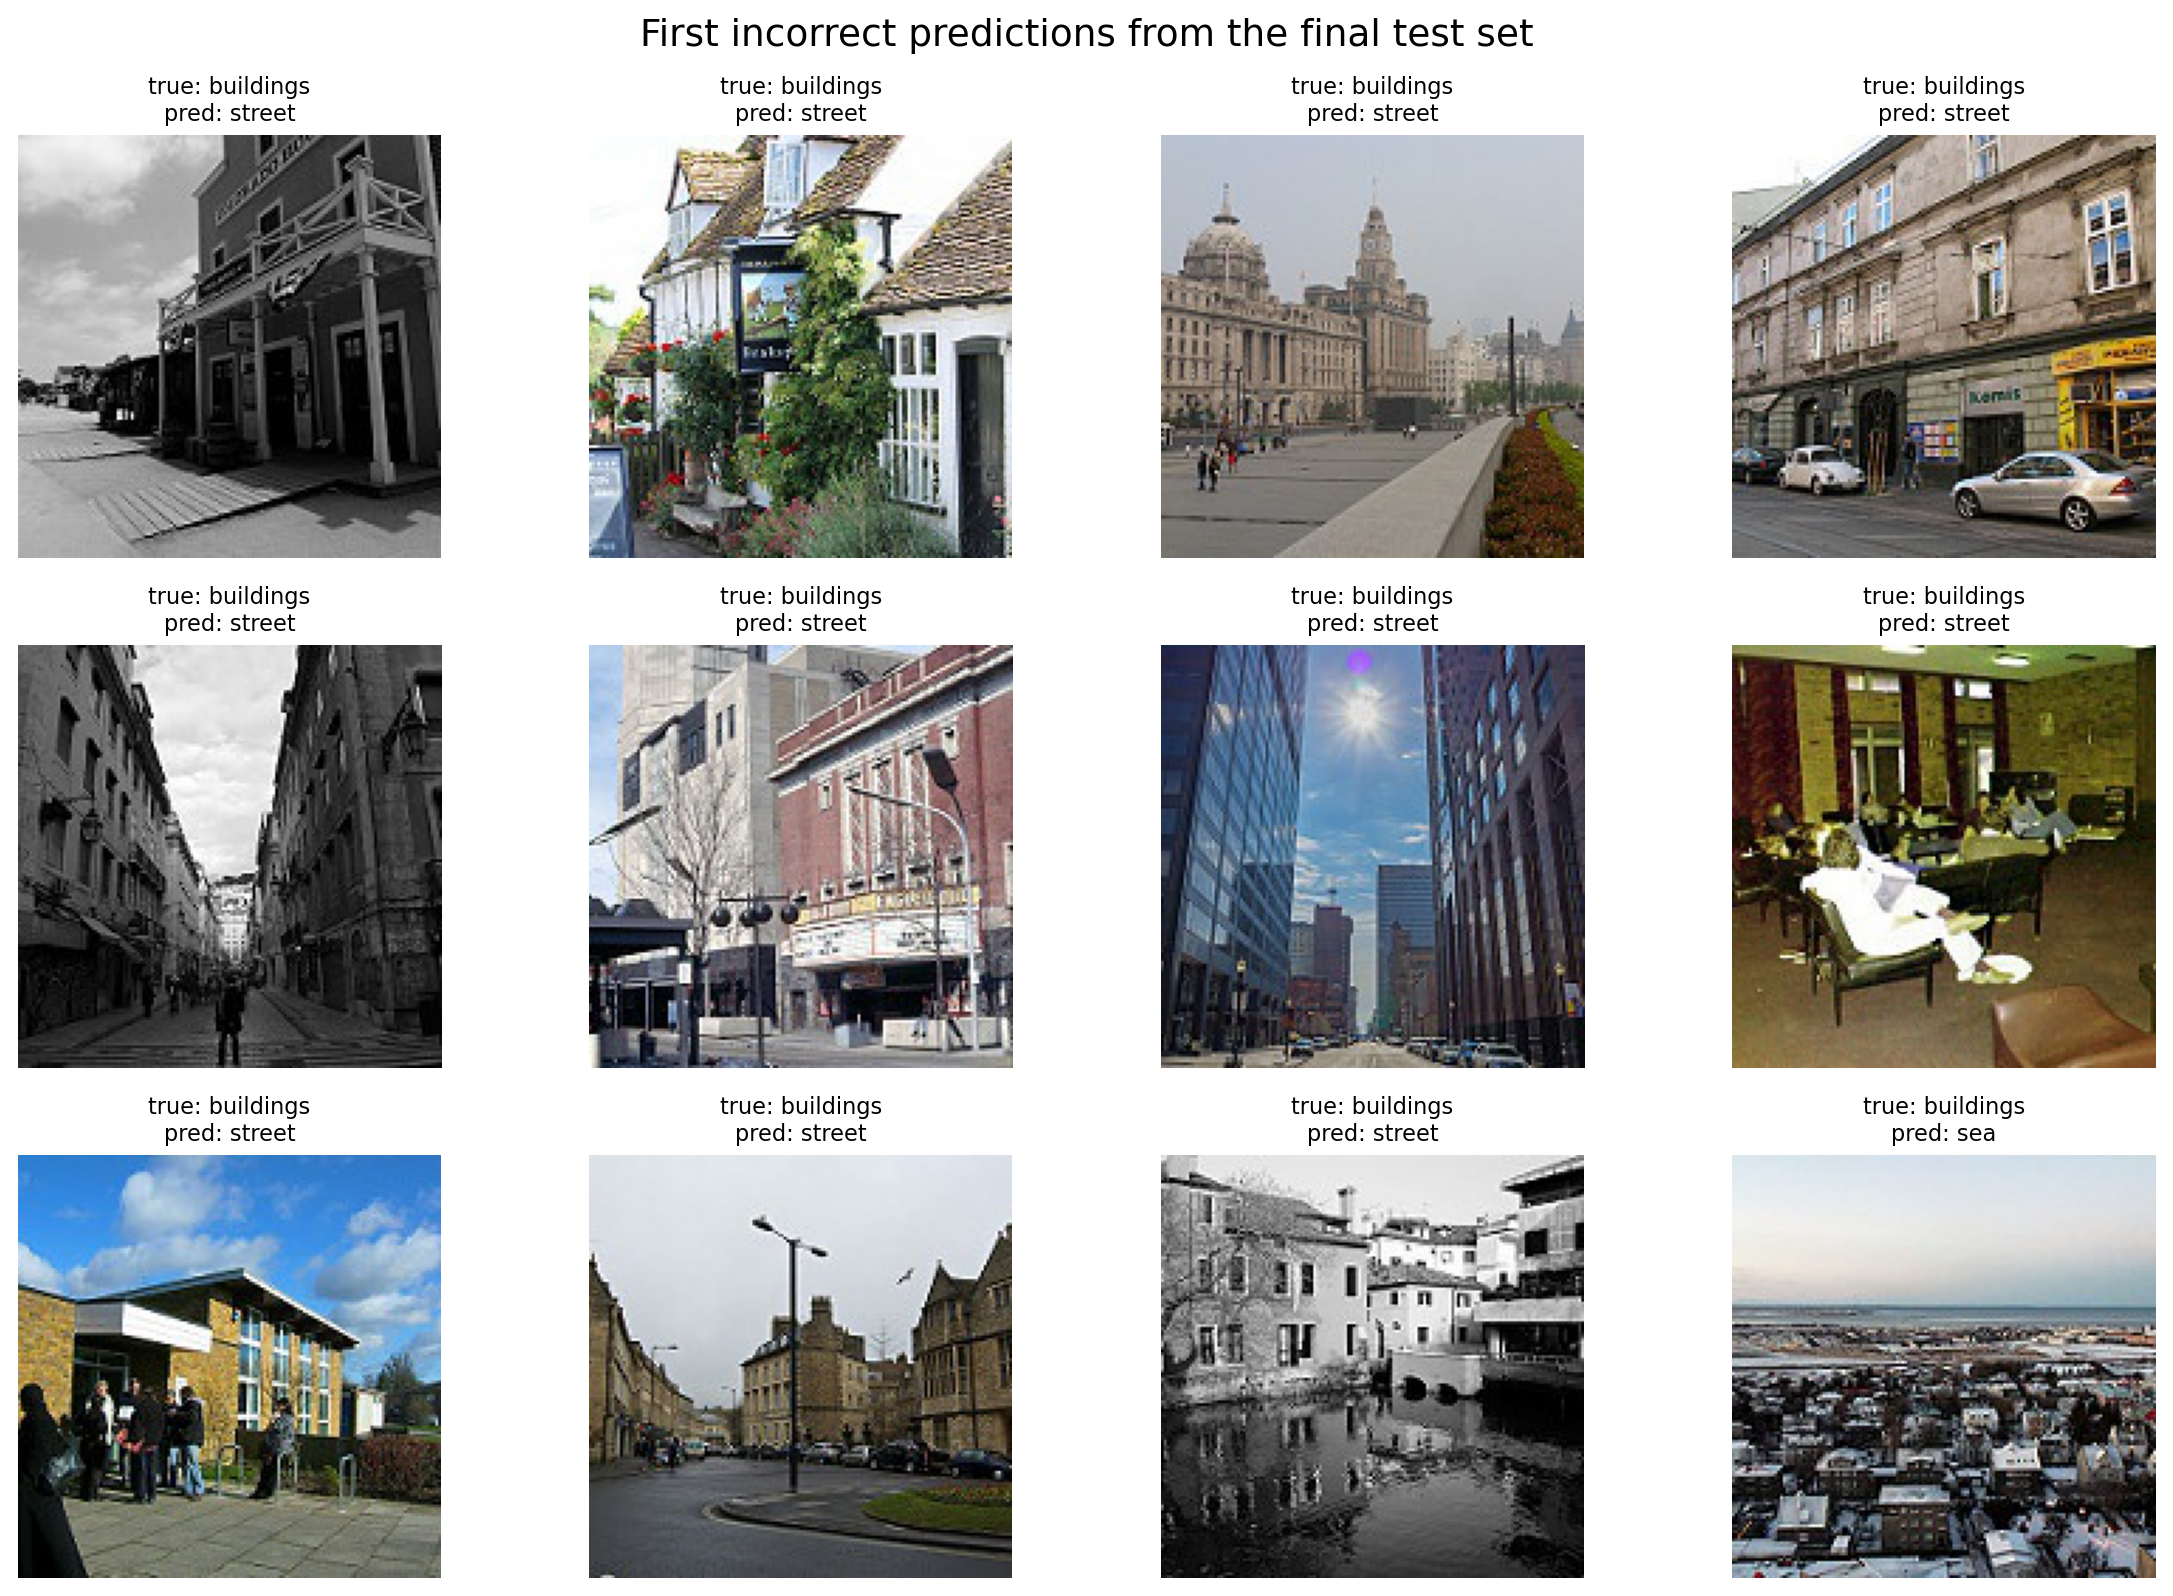
\includegraphics[width=\textwidth]{images/intel_08_error_examples.png}
\caption{Twelve incorrect predictions from the selected model on the untouched source test set.}
\label{fig:intel-errors}
\end{figure}

\begin{importantbox}
\textbf{Image conclusion.} Pretrained MobileNetV3-Small features plus balanced Logistic Regression are a strong, simple, and reproducible baseline for Intel scene classification. The result meets the assignment workflow because EDA, augmentation, a pretrained deep representation, a validation comparison, and a final untouched test evaluation are all present. It is still a classroom model: it can confuse visually related scenes and should not be treated as a general-purpose real-world scene understanding system.
\end{importantbox}

\iffalse
\section{Image Data: Galaxy10 DECaLS Galaxy Morphology}
\label{sec:image}

\subsection{Task Objective and Dataset}

The image task classifies one astronomical cutout into one of ten visual morphology labels. The selected dataset is Galaxy10 DECaLS NoDuplicated \cite{galaxy10}. It contains 17,675 colour images of size 256 by 256 pixels. The three visible channels are created from the DECaLS survey bands. The task is useful for a first image-classification exercise because every observation has the same image size, but the visual shapes remain varied and difficult.

The label is a morphology category, such as \textit{Round smooth}, \textit{Barred spiral}, or \textit{Edge-on with bulge}. These labels describe the visual appearance used in the dataset. They are not a new scientific confirmation produced by this project. The model learns to reproduce the provided label from pixels, and the final score measures agreement with those held-out labels.

The HDF5 file also contains right ascension, declination, redshift, and pixel scale. These fields are useful for inspecting the source dataset, but they are not model inputs. The purpose of this task is image classification, so using astronomical metadata would make the answer depend on information outside the image. The notebook therefore uses only the RGB pixel array and the supplied class label.

\subsubsection{Dataset Structure and Class Balance}

The working file contains the HDF5 keys \texttt{images}, \texttt{ans}, \texttt{ra}, \texttt{dec}, \texttt{redshift}, and \texttt{pxscale}. The \texttt{images} key has shape $(17{,}675, 256, 256, 3)$ and unsigned 8-bit values from 0 to 255. The \texttt{ans} key is the integer class label. The notebook checks the official MD5 hash before loading the file; this prevents an interrupted download from silently entering the analysis.

Figure~\ref{fig:image-examples} shows one randomly selected image from each class using the fixed seed. The examples make the task concrete. Some objects are bright and centred, while others are faint, surrounded by unrelated sources, or have a visible neighbour. These background objects and changes in brightness are part of the reason that morphology classes can be confused.

\begin{figure}[H]
\centering
\includegraphics[width=\textwidth]{images/image_01_class_examples.png}
\caption{One Galaxy10 DECaLS image from each of the 10 morphology classes. The visual category is the supplied target label.}
\label{fig:image-examples}
\end{figure}

Table~\ref{tab:image-class-counts} and Figure~\ref{fig:image-distribution} show that the classes are not equally frequent. \textit{Cigar shaped} is the smallest class with only 333 images (1.88\%), while \textit{Round smooth} and \textit{Unbarred loose spiral} each contain about 15\% of the dataset. For this reason, the report uses balanced accuracy and macro F1 in addition to ordinary accuracy. These metrics prevent a large class from dominating the evaluation.

\begin{table}[H]
\centering
\caption{Galaxy10 DECaLS class distribution.}
\label{tab:image-class-counts}
\small
\begin{tabular}{lr r}
\toprule
\textbf{Morphology class} & \textbf{Images} & \textbf{Share} \\
\midrule
Disturbed & 1,081 & 6.12\% \\
Merging & 1,853 & 10.48\% \\
Round smooth & 2,640 & 14.94\% \\
In-between round & 2,021 & 11.43\% \\
Cigar shaped & 333 & 1.88\% \\
Barred spiral & 2,040 & 11.54\% \\
Unbarred tight spiral & 1,823 & 10.31\% \\
Unbarred loose spiral & 2,600 & 14.71\% \\
Edge-on without bulge & 1,419 & 8.03\% \\
Edge-on with bulge & 1,865 & 10.55\% \\
\bottomrule
\end{tabular}
\end{table}

\begin{figure}[H]
\centering
\begin{minipage}{0.52\textwidth}
\centering
\includegraphics[width=\textwidth]{images/image_02_class_distribution.png}\\
\small (a) Image count by class
\end{minipage}\hfill
\begin{minipage}{0.43\textwidth}
\centering
\includegraphics[width=\textwidth]{images/image_03_brightness_by_class.png}\\
\small (b) Brightness from 100 images per class
\end{minipage}
\caption{Image-level EDA. The brightness plot is a balanced inspection sample, not a model feature.}
\label{fig:image-distribution}
\end{figure}

The brightness box plot uses at most 100 images from every class, so a common class cannot fill the plot by itself. It confirms that image brightness varies inside and across classes. The plot is not used to make a scientific statement about galaxies, and it is not inserted as a separate numerical feature. It is a simple quality check that supports using normalization before the pretrained network.

\subsubsection{Data Quality and Leakage Control}

The selected release is called \textit{NoDuplicated}, which reduces the risk of exact duplicate images appearing across the split. The redshift field has 92 missing values, but this does not affect the model because redshift is excluded from the input. Pixel scale has no missing values. A separate image-level split is still needed: seeing a test image during training would make the test score unfair even when every image file is unique.

\begin{table}[H]
\centering
\caption{Image-task data-quality and leakage decisions.}
\label{tab:image-quality}
\begin{tabularx}{\textwidth}{lX}
\toprule
\textbf{Check} & \textbf{Decision and reason} \\
\midrule
File integrity & The official MD5 hash is checked before HDF5 loading. A mismatched file stops the notebook. \\
Duplicate risk & The NoDuplicated release is used. Train, validation, and test use different image indices. \\
Missing metadata & 92 redshift values are missing; redshift is inspected only and never enters the image model. \\
Input leakage & Right ascension, declination, redshift, pixel scale, and target names are excluded from model inputs. \\
Model selection & Validation macro F1 selects the final model. The test set is evaluated only after this choice. \\
\bottomrule
\end{tabularx}
\end{table}

\subsection{Preprocessing, Split, and Augmentation}

The dataset has no predefined train, validation, and test partitions. The notebook first splits image indices using a fixed random seed of 42. It uses 70\% for training, then divides the remaining 30\% equally into validation and test sets. Stratification preserves the 10 label proportions in every partition. Table~\ref{tab:image-split} shows the result.

\begin{table}[H]
\centering
\caption{Stratified split used for the Galaxy10 task.}
\label{tab:image-split}
\begin{tabular}{lr r}
\toprule
\textbf{Split} & \textbf{Images} & \textbf{Purpose} \\
\midrule
Training & 12,372 & Fit Logistic Regression and the small classifier head \\
Validation & 2,651 & Compare models and choose the final model \\
Test & 2,652 & One final evaluation after selection \\
\bottomrule
\end{tabular}
\end{table}

MobileNetV3-Small was pretrained with ImageNet images. Each Galaxy10 image is therefore resized from 256 by 256 to 160 by 160 pixels, converted to a tensor, and normalized by the ImageNet channel mean and standard deviation. This does not change the target label; it changes the numerical scale of pixels into the scale expected by the pretrained model.

Training images also receive a random horizontal flip. A left-right flip does not change whether a galaxy is spiral, smooth, or edge-on. The same flip is not used on validation or test images, so their predictions are deterministic. Figure~\ref{fig:image-preprocessing} shows the augmentation and the five-epoch learning history of the frozen MobileNetV3 head.

\begin{figure}[H]
\centering
\begin{minipage}{0.42\textwidth}
\centering
\includegraphics[width=\textwidth]{images/image_04_augmentation_example.png}\\
\small (a) Horizontal-flip augmentation
\end{minipage}\hfill
\begin{minipage}{0.53\textwidth}
\centering
\includegraphics[width=\textwidth]{images/image_05_training_history.png}\\
\small (b) Frozen-head learning history
\end{minipage}
\caption{Preprocessing and training checks. The head improves during five epochs but remains below the Logistic Regression baseline.}
\label{fig:image-preprocessing}
\end{figure}

\subsection{Model Comparison}

Two simple approaches use the same MobileNetV3-Small pretrained weights. The first approach freezes the entire network and converts each image into a 576-value feature vector. Logistic Regression with balanced class weights is fitted on the training vectors. This is the baseline because it is easy to understand: the pretrained network describes the image, then a linear classifier chooses a morphology label.

The second approach also starts from pretrained MobileNetV3-Small, freezes its feature layers, and replaces the final classifier with a small head: a 256-unit linear layer, Hardswish activation, 0.2 dropout, and a 10-unit output layer. Only 150,282 head parameters are trainable. Class-weighted cross-entropy and Adam with learning rate 0.0003 are used for five epochs. This is transfer learning because ImageNet visual features are reused while the new head learns the Galaxy10 labels.

Table~\ref{tab:image-validation} and Figure~\ref{fig:image-models} compare both approaches on validation data. The pretrained feature vectors plus Logistic Regression have the higher macro F1 (0.5952 versus 0.4357), so this model is selected before viewing the final test score. The frozen head is retained as a required deep-learning comparison, but it is not presented as the better result.

\begin{table}[H]
\centering
\caption{Validation comparison. The selected model has the highest macro F1.}
\label{tab:image-validation}
\begin{tabular}{lrrr}
\toprule
\textbf{Model} & \textbf{Accuracy} & \textbf{Balanced acc.} & \textbf{Macro F1} \\
\midrule
Pretrained features + Logistic & \textbf{0.6175} & \textbf{0.6141} & \textbf{0.5952} \\
Frozen MobileNetV3 head & 0.4594 & 0.4619 & 0.4357 \\
\bottomrule
\end{tabular}
\end{table}

\begin{figure}[H]
\centering
\includegraphics[width=0.80\textwidth]{images/image_06_model_comparison.png}
\caption{Validation scores for the two pretrained-image approaches.}
\label{fig:image-models}
\end{figure}

\subsection{Final Test Results and Error Review}

The selected model is evaluated once on 2,652 test images. It obtains accuracy 0.5984, balanced accuracy 0.5990, and macro F1 0.5797. The three numbers are close because the classifier does not obtain its score only from a large class. The test macro F1 is slightly lower than validation macro F1, which is expected when a selected model is evaluated on previously unseen images.

The normalized confusion matrix in Figure~\ref{fig:image-confusion} is read row by row. A row is one true class, and the diagonal cell is the recall for that class. The best recalls are 0.826 for \textit{Edge-on without bulge} and 0.782 for \textit{Edge-on with bulge}. \textit{Unbarred loose spiral} has the lowest recall, 0.369. It is often confused with other spiral classes, which is reasonable because the boundary between a loose arm, a tight arm, and a bar can be unclear in a small noisy cutout.

\begin{figure}[H]
\centering
\includegraphics[width=0.91\textwidth]{images/image_07_confusion_matrix.png}
\caption{Normalized test confusion matrix for the selected pretrained-feature Logistic Regression model.}
\label{fig:image-confusion}
\end{figure}

Table~\ref{tab:image-errors} lists the most frequent directional errors. For example, 64 true \textit{Unbarred loose spiral} images are predicted as \textit{Unbarred tight spiral}. This does not prove that a label is wrong. It shows that the learned pretrained features and simple linear boundary are not sufficient to separate all visual subtypes reliably.

\begin{table}[H]
\centering
\caption{Most frequent wrong test predictions.}
\label{tab:image-errors}
\begin{tabular}{llr}
\toprule
\textbf{True label} & \textbf{Predicted label} & \textbf{Images} \\
\midrule
Unbarred loose spiral & Unbarred tight spiral & 64 \\
In-between round & Round smooth & 52 \\
Unbarred loose spiral & Barred spiral & 52 \\
Barred spiral & Unbarred loose spiral & 51 \\
Unbarred loose spiral & Disturbed & 48 \\
Barred spiral & Unbarred tight spiral & 45 \\
Round smooth & In-between round & 43 \\
\bottomrule
\end{tabular}
\end{table}

Figure~\ref{fig:image-errors} shows the first 12 incorrect test images, with true and predicted labels above each cutout. Several cases contain a small or faint target, bright nearby objects, or visual features shared by several classes. These are useful concrete examples of why a moderate macro F1 should not be interpreted as reliable automated morphology labelling.

\begin{figure}[H]
\centering
\includegraphics[width=\textwidth]{images/image_08_error_examples.png}
\caption{Twelve incorrect predictions from the selected model on the held-out test set.}
\label{fig:image-errors}
\end{figure}

\begin{importantbox}
\textbf{Image conclusion.} Pretrained MobileNetV3 feature vectors plus balanced Logistic Regression are a clear and reproducible first baseline for Galaxy10 DECaLS. The model recognizes edge-on and round categories relatively well, but it still confuses visually related spiral and disturbed classes. The result is suitable for learning image EDA and fair evaluation; it is not a substitute for expert astronomical morphology analysis.
\end{importantbox}

\fi
\section{Overall Conclusion}

The three tasks show the same lesson: EDA changes model decisions. The same general workflow is used in every task, but the details must be adapted to the data type. For KOI records, one row contains measured numerical and categorical properties of one astronomical object. The key risks are missing measurements, skewed values, and fields that reveal the final catalogue decision. For comments, one row contains a variable-length sentence. The key risks are repeated normalized text, an imbalanced toxic class, and wording that has a meaning only in context. For Intel scenes, one observation is a pixel image. The key risks are class imbalance, brightness and background variation, train--test leakage, and visually similar scenes such as glacier and mountain.

The analysis framework is therefore simple but explicit. First, inspect the target, size, missing values, duplicates, and distributions. Second, define what information is allowed as input and remove direct leakage. Third, prepare the input using rules learned from training data only. Fourth, compare a small baseline with one stronger but still understandable model on validation data. Finally, use the test set once and inspect errors instead of relying on one headline score. These steps make the result easier to check and reduce the chance that a score is improved by an unfair shortcut.

\subsection{Summary of Final Results}

The final results are summarized below. Accuracy counts all correct predictions. Balanced accuracy checks whether every class is recognized fairly. Macro F1 balances precision and recall for each class before averaging them. For this reason, macro F1 is the most useful single comparison measure in this report, especially for the imbalanced toxicity task, the three-class KOI task, and the 10-class image task.

\begin{table}[H]
\centering
\caption{Final selected-model results.}
\label{tab:final-results}
\resizebox{\textwidth}{!}{%
\begin{tabular}{llrrr}
\toprule
\textbf{Task} & \textbf{Selected model} & \textbf{Accuracy} & \textbf{Balanced acc.} & \textbf{Macro F1} \\
\midrule
Kepler KOI & Balanced Random Forest & 0.758 & 0.730 & 0.727 \\
ViCTSD Toxicity & Word TF-IDF + Logistic & 0.842 & 0.732 & 0.679 \\
ViCTSD Constructiveness & Word TF-IDF + Logistic & 0.807 & 0.812 & 0.800 \\
Intel Image Classification & Pretrained features + Logistic & 0.914 & 0.916 & 0.916 \\
\bottomrule
\end{tabular}
}
\end{table}

\subsection{Limitations and Future Work}

The code is deliberately compact and beginner-friendly. This makes the workflow easier to reproduce, but it also creates clear limits. The KOI model uses a fixed set of catalogue variables and a simple group split; it cannot replace scientific confirmation from physical follow-up observations. The text model has no sentence-level understanding of sarcasm, conversation history, or implied meaning. Its predictions should be treated as model suggestions, not final moderation decisions. The Galaxy10 model observes only image pixels and was compared with a small frozen head for five epochs. It can confuse faint, crowded, or visually similar morphology classes and cannot replace expert inspection.

Future work may add carefully designed KOI features, compare different group-aware resampling seeds, or calibrate predicted probabilities. For text, later experiments may use Vietnamese word segmentation, a pretrained Vietnamese language model, or human review of important error groups. For images, later work may carefully fine-tune more MobileNetV3 layers, test additional valid augmentations, or review error groups with an astronomy expert. Each improvement would need to repeat the same leakage checks and keep the test split independent. These are possible next experiments, not results claimed by the current report.

\section*{Reproducibility}
\addcontentsline{toc}{section}{Reproducibility}
The following project files can reproduce the analysis. A simple order is: install the notebook requirements, place the data files in the stated data folder, run the tabular notebook from top to bottom, then run the text notebook, and finally run the image notebook. The notebooks create the tables and figures used by the report. Re-running a model with the documented random seed makes the split and the main reported results repeatable in the same software environment.
\begin{itemize}[leftmargin=5mm]
  \item \texttt{notebooks/tabular\_koi\_eda.ipynb} for the Kepler KOI task.
  \item \texttt{notebooks/text\_victsd\_eda.ipynb} for the ViCTSD task.
  \item \texttt{notebooks/image\_intel\_eda.ipynb} for the Intel Image Classification task.
  \item \texttt{data/koi\_cumulative.csv}, the three \texttt{data/victsd\_*.csv} files, and public source folders downloaded by the image notebook.
  \item \texttt{reports/figures/} for the generated figures.
  \item The Intel JSON summary and test-prediction CSV in \texttt{reports/} for the selected image-model result.
\end{itemize}

\clearpage
\begin{thebibliography}{9}
\bibitem{assignment-vne}
Le Thanh Sach. \textit{Programming Foundation for Data Analytics and Visualization: Course Project Assignment, Version 4.0}. Ho Chi Minh City University of Technology, Semester 261, September 2026.

\bibitem{nasa-koi}
NASA Exoplanet Archive. \textit{Kepler Objects of Interest Cumulative Table}. Available at: \url{https://exoplanetarchive.ipac.caltech.edu/docs/Kepler_KOI_docs.html}. Accessed October 2026.

\bibitem{victsd}
tarudesu. \textit{ViCTSD: Vietnamese Constructive and Toxic Speech Detection}. GitHub repository. Available at: \url{https://github.com/tarudesu/ViCTSD}. Accessed October 2026.

\bibitem{intel}
Puneet6060. \textit{Intel Image Classification}. Kaggle dataset. Available at: \url{https://www.kaggle.com/datasets/puneet6060/intel-image-classification}. Accessed October 2026.

\end{thebibliography}

\end{document}
